\section{Giới thiệu}
\hspace{1cm} Ngành công nghiệp trò chơi điện tử (game) đã và đang trải qua một giai đoạn bùng nổ mạnh mẽ, trở thành một trong những lĩnh vực giải trí mang lại doanh thu khổng lồ trên toàn cầu. Sự phát triển không ngừng của công nghệ đồ họa, phần cứng cũng như sự thay đổi trong thói quen giải trí của người dùng đã định hình lại toàn bộ bức tranh của ngành. Trong số các nền tảng phân phối game hiện nay, Steam nổi lên như một hệ sinh thái lớn nhất dành cho game PC, lưu trữ dữ liệu của hàng trăm ngàn tựa game và hàng triệu lượt đánh giá từ cộng đồng người chơi.

\hspace{1cm} Tuy nhiên, sự phát triển bùng nổ cũng đi kèm với mức độ cạnh tranh khốc liệt. Hàng năm, có hàng ngàn tựa game mới được phát hành, nhưng chỉ một phần nhỏ trong số đó gặt hái được thành công và tiếp cận được tệp khách hàng rộng lớn. Phần lớn các studio phát triển game, đặc biệt là các studio độc lập (indie studios), thường gặp khó khăn trong việc nắm bắt thị hiếu người dùng, định giá sản phẩm và lựa chọn hướng đi công nghệ phù hợp.

\hspace{1cm} Nắm bắt được những thách thức đó, việc ứng dụng Khai phá dữ liệu (Data Mining) và Học máy (Machine Learning) để phân tích tập dữ liệu lịch sử của ngành game đang mở ra một giải pháp chiến lược. Trong khuôn khổ của bài báo cáo này, nhóm tập trung vào việc giải quyết bài toán "Phân tích xu hướng phát triển của ngành trò chơi điện tử" với các mục tiêu cụ thể như sau:
\begin{itemize}
    \item Vấn đề cốt lõi: Làm thế nào để dự đoán được tiềm năng thành công của một tựa game trước khi phát hành, cũng như hiểu rõ các yếu tố nào ảnh hưởng mạnh mẽ nhất đến sự phổ biến của nó trên thị trường.
    \item Giải pháp khai phá dữ liệu: Ứng dụng các thuật toán Khai phá dữ liệu để tìm ra các mẫu tiềm ẩn (patterns) trong các đặc trưng của game như thể loại, giá bán, nền tảng hỗ trợ và mô tả.
    \item Mục tiêu bài toán: Phân tích xu hướng phát triển của ngành công nghiệp game qua các giai đoạn, từ đó đưa ra định hướng chiến lược cho các studio lập trình game.
    \item Bộ dữ liệu sử dụng: Đề tài được thực hiện trên tập dữ liệu khổng lồ bao gồm hơn 122.000 trò chơi điện tử được phát hành trên nền tảng Steam trong giai đoạn từ năm 1997 đến năm 2025.
\end{itemize}

\hspace{1cm} Từ mục tiêu và bộ dữ liệu đã xác định, phần tiếp theo sẽ cung cấp cái nhìn tổng quan về quy trình thực hiện, từ tiền xử lý dữ liệu khám phá đến xây dựng và đánh giá các mô hình học máy.






\newpage
\section{Tổng quan công việc}

\subsection{Giới thiệu về phương pháp luận}
\hspace{1cm} Bài báo cáo này áp dụng phương pháp luận thực nghiệm theo quy trình chuẩn của Khai phá dữ liệu (KDD - Knowledge Discovery in Databases). Trọng tâm của phương pháp luận là khai thác đa chiều bộ dữ liệu thông qua ba nhóm bài toán chính: Phân loại (Classification), Gom cụm (Clustering) và Khai phá luật kết hợp (Association Rules Mining).

\subsection{Phương pháp tiếp cận}
\hspace{1cm} Để giải quyết bài toán, nhóm đã áp dụng phương pháp tiếp cận theo 4 bước chính:
\begin{enumerate}
    \item Tìm hiểu và tiền xử lý dữ liệu: Tiến hành làm sạch tập dữ liệu lớn bằng cách loại bỏ các cột không mang ý nghĩa phân tích, xử lý các tựa game có mô tả bị lỗi font (Tiếng Trung) và chuẩn hóa các trường dữ liệu dạng chuỗi về định dạng có thể tính toán được.
    \item Lựa chọn và xây dựng mô hình: Dựa trên yêu cầu phân tích, nhóm thiết lập các mô hình:
    \begin{itemize}
        \item Classification: Sử dụng Decision Tree, Random Forest, SVM để dự đoán sự thành công của game (trên 200.000 lượt sở hữu).
        \item Clustering: Sử dụng K-Means, DBSCAN để phân nhóm các tựa game tương tự, tìm kiếm phân khúc thị trường.
        \item Association Rules: Sử dụng Apriori để tìm các thể loại thường xuyên xuất hiện cùng nhau.
    \end{itemize}
    \item Khám phá xu hướng: Kết hợp các kỹ thuật trực quan hóa dữ liệu (Data Visualization) để chỉ ra nguyên nhân của sự phát triển và các đỉnh điểm bùng nổ trên đồ thị thời gian.
    \item Đánh giá và định hướng: Rút ra các kết luận logic để tư vấn trực tiếp cho các nhà phát triển game.
\end{enumerate}

\subsection{Các kỹ thuật sử dụng}
\hspace{1cm} Các công cụ và thư viện chính được sử dụng bao gồm:
\begin{itemize}
    \item Thư viện chính: Pandas và Numpy (để xử lý dữ liệu ma trận và làm sạch dữ liệu), Matplotlib và Seaborn (để vẽ biểu đồ phân phối, biểu đồ nhiệt) và Scikit-learn (cho việc xây dựng mô hình).
    \item Tiền xử lý văn bản: Sử dụng biểu thức chính quy (\texttt{regex}) để phát hiện và loại bỏ các ký tự CJK (Chinese, Japanese, Korean) không hợp lệ trong mô tả.
    \item Phân rã dữ liệu: Phân tách các chuỗi thể loại (\texttt{Genres}) chứa nhiều giá trị thành các biến độc lập để đếm tần suất.
\end{itemize}







\newpage
\section{Cơ sở lý thuyết}

\subsection{Phân tích dữ liệu khám phá (Exploratory Data Analysis - EDA)}
\hspace{1cm} Phân tích dữ liệu khám phá (EDA) là bước đầu tiên và mang tính nền tảng trong bất kỳ quy trình khai phá dữ liệu nào. Đối với ngành công nghiệp trò chơi điện tử, EDA giúp nhận diện các mẫu (patterns) cơ bản, các bất thường (outliers) và các xu hướng tổng quan trước khi áp dụng các mô hình học máy phức tạp. Mục tiêu của giai đoạn này là đưa ra được xu hướng phát triển của ngành game qua từng giai đoạn , chỉ ra nguyên nhân của sự phát triển cũng như các đỉnh trên đồ thị và đưa ra các yếu tố ảnh hưởng đến sự phổ biến của 1 tựa game.

\hspace{1cm} Cụ thể, thông qua EDA, các yếu tố cốt lõi định hình thị trường được làm rõ. Về mặt giá cả, phân tích tập trung vào tỷ lệ game miễn phí so với game trả phí ở từng nhóm độ phổ biến, giúp đánh giá hiệu quả của mô hình kinh doanh Free-to-Play. Về mặt kỹ thuật, tỷ lệ hỗ trợ đa nền tảng (Windows, Mac, Linux) được phân tích để xem xét mức độ mở rộng tệp khách hàng. Ngoài ra, các chỉ số về tỷ lệ đánh giá tích cực (Positive Reviews) và chiều dài của đoạn văn bản mô tả game cũng được thống kê chi tiết nhằm tìm ra mối tương quan với mức độ thành công của tựa game trên thị trường.

\subsection{Bài toán Phân loại (Classification)}
\hspace{1cm} Phân loại (Classification) là một kỹ thuật học máy có giám sát, trong đó mô hình học cách gán một nhãn phân lớp cho các quan sát mới dựa trên tập dữ liệu huấn luyện đã được gán nhãn trước. Trong phân tích dữ liệu game, các thuật toán phân loại được ứng dụng để giải quyết nhiều mục tiêu quan trọng như: dự đoán game sẽ thành công (đạt mức 200K+ người sở hữu) dựa trên giá, thể loại, hệ điều hành hỗ trợ, độ dài mô tả và số lượng DLC ; phân loại game vào các nhóm độ phổ biến khác nhau từ 0-20K cho đến 100M-200M ; và dự đoán xu hướng đánh giá (tích cực/tiêu cực) từ các đặc điểm của game.

\hspace{1cm} Để giải quyết các bài toán trên, nghiên cứu xem xét ứng dụng đa dạng các thuật toán phân loại mạnh mẽ:
\begin{itemize}
    \item \textbf{Cây quyết định (Decision Tree):} Mô hình hóa các quyết định dưới dạng một cấu trúc cây, trong đó mỗi nút nội bộ đại diện cho một kiểm tra trên một thuộc tính (ví dụ: Giá có nhỏ hơn 10\$ không?), và mỗi nhánh đại diện cho kết quả của kiểm tra đó. Thuật toán này có ưu điểm là rất trực quan và dễ diễn giải các quy luật kinh doanh.
    \item \textbf{Rừng ngẫu nhiên (Random Forest):} Là một phương pháp học tập tập hợp (ensemble learning) hoạt động bằng cách xây dựng vô số các cây quyết định trong thời gian huấn luyện. Phương pháp này giúp khắc phục nhược điểm dễ bị quá khớp (overfitting) của một cây quyết định đơn lẻ, mang lại độ chính xác và tính ổn định cao hơn.
    \item \textbf{Máy véctơ hỗ trợ (SVM - Support Vector Machine):} Hoạt động bằng cách tìm ra một siêu phẳng (hyperplane) trong không gian $N$-chiều để phân tách các điểm dữ liệu thuộc các lớp khác nhau với biên độ (margin) lớn nhất có thể.
\end{itemize}

\subsection{Bài toán gom cụm (Clustering)}
\hspace{1cm} Trái ngược với phân loại, gom cụm (Clustering) là một kỹ thuật học máy không giám sát. Mục tiêu của nó là nhóm một tập hợp các đối tượng sao cho các đối tượng trong cùng một cụm (cluster) có tính tương đồng cao hơn so với các đối tượng thuộc các cụm khác. Kỹ thuật này được ứng dụng để nhóm các game tương tự nhau dựa trên giá, thể loại, và các lượt đánh giá nhằm tìm ra các phân khúc thị trường (market segments) cho các studio độc lập (indie studios) , đồng thời phân tích xem các tựa game thành công thường có chung những đặc điểm gì.

\hspace{1cm} Các thuật toán gom cụm tiêu biểu được nghiên cứu bao gồm:
\begin{itemize}
    \item \textbf{K-Means:} Thuật toán phân chia tập dữ liệu thành $K$ cụm khác biệt và không chồng chéo. Thuật toán cố gắng giảm thiểu phương sai trong mỗi cụm, giúp tìm ra các nhóm game có tính chất hội tụ rõ ràng (ví dụ: nhóm game giá rẻ, chơi ngắn, đánh giá trung bình).
    \item \textbf{DBSCAN (Density-Based Spatial Clustering of Applications with Noise):} Thuật toán gom cụm dựa trên mật độ, có khả năng tìm ra các cụm với hình dạng tùy ý và tự động cô lập các điểm dữ liệu nhiễu (outliers).
    \item \textbf{Gom cụm phân cấp (Hierarchical Clustering):} Xây dựng một hệ thống phân cấp các cụm dưới dạng biểu đồ cây (dendrogram), cho phép các nhà phân tích quan sát được sự hợp nhất hoặc phân chia của các thể loại game ở nhiều mức độ chi tiết khác nhau.
    \item \textbf{Mô hình hỗn hợp Gaussian (GMM - Gaussian Mixture Models):} Một phương pháp tiếp cận xác suất, giả định rằng tất cả các điểm dữ liệu được sinh ra từ một hỗn hợp của một số hữu hạn các phân phối Gaussian, cho phép việc gom cụm linh hoạt hơn bằng cách gán xác suất (soft-clustering) cho mỗi điểm dữ liệu thay vì gán cứng như K-Means.
\end{itemize}

\subsection{Khai phá luật kết hợp (Association Rules Mining)}
\hspace{1cm} Khai phá luật kết hợp là phương pháp khám phá các mối quan hệ thú vị và các mẫu thường xuyên (frequent patterns) ẩn sâu trong các cơ sở dữ liệu lớn. Ứng dụng chính của kỹ thuật này trong ngành game là tìm ra các thể loại (genres) thường đi kèm với nhau (ví dụ: Action thường kết hợp với Adventure) , đồng thời tìm kiếm mối quan hệ giữa các danh mục (Categories) và thẻ (Tags), từ đó phát hiện ra các mẫu như việc game có lượng DLC lớn cộng với việc hỗ trợ hệ điều hành Mac thường đi đôi với mức giá bán cao hơn.

\hspace{1cm} Các thuật toán khai phá luật kết hợp được xem xét sử dụng bao gồm:
\begin{itemize}
    \item \textbf{Thuật toán Apriori:} Đây là thuật toán kinh điển nhất, hoạt động dựa trên nguyên lý tiên nghiệm: "Nếu một tập mục là phổ biến, thì tất cả các tập con của nó cũng phải phổ biến". Thuật toán quét cơ sở dữ liệu nhiều lần để đếm tần suất, từ đó sinh ra các luật dựa trên các ngưỡng Hỗ trợ (Support) và Độ tin cậy (Confidence).
    \item \textbf{Thuật toán FP-Growth (Frequent Pattern Growth):} Khắc phục nhược điểm phải quét dữ liệu nhiều lần của Apriori. FP-Growth nén cơ sở dữ liệu thành một cấu trúc cây (FP-Tree), sau đó tiến hành khai phá trực tiếp trên cây này, giúp tăng tốc độ xử lý một cách đáng kể khi đối mặt với bộ dữ liệu khổng lồ gồm hơn 122.000 trò chơi của nền tảng Steam.
\end{itemize}



\newpage
\section{Mô tả bộ dữ liệu}

\subsection{Nguồn dữ liệu}
\hspace{1cm} Tập dữ liệu được sử dụng trong bài nghiên cứu là "Steam Games Dataset", được thu thập và công bố trên nền tảng Kaggle. Tập dữ liệu này bao gồm thông tin chi tiết của hơn 122.000 trò chơi điện tử được phát hành trên nền tảng phân phối game Steam trong khoảng thời gian từ năm 1997 đến năm 2025. Đây là một trong những kho dữ liệu đồ sộ và toàn diện nhất về ngành công nghiệp game trên PC, cung cấp góc nhìn sâu sắc về vòng đời, mức độ phổ biến, phản hồi từ cộng đồng và chiến lược kinh doanh của các tựa game.



\subsection{Các đặc trưng của dữ liệu}
\hspace{1cm} Bộ dữ liệu gốc bao gồm 39 đặc trưng (cột), cung cấp thông tin đa chiều về mỗi tựa game. Để thuận tiện cho quá trình phân tích và huấn luyện mô hình học máy, các đặc trưng này được phân thành các nhóm chính như sau:

\begin{itemize}
    \item \textbf{Thông tin định danh và cơ bản:}
    \begin{itemize}
        \item \texttt{AppID}: Mã định danh duy nhất của trò chơi trên hệ thống Steam.
        \item \texttt{Name}: Tên chính thức của trò chơi.
        \item \texttt{Release date}: Ngày phát hành chính thức.
        \item \texttt{Developers} và \texttt{Publishers}: Tên đội ngũ phát triển và nhà phát hành game.
        \item \texttt{Required age}: Độ tuổi tối thiểu được yêu cầu để chơi game.
    \end{itemize}

    \item \textbf{Chỉ số thương mại và giá cả:}
    \begin{itemize}
        \item \texttt{Price}: Giá bán lẻ của tựa game (tính bằng USD).
        \item \texttt{Discount}: Mức giảm giá hiện tại (nếu có).
        \item \texttt{DLC count}: Số lượng bản mở rộng (Downloadable Content) đi kèm.
    \end{itemize}

    \item \textbf{Độ phổ biến và mức độ tương tác:}
    \begin{itemize}
        \item \texttt{Estimated owners}: Khoảng ước tính số lượng người dùng sở hữu tựa game.
        \item \texttt{Peak CCU}: Số lượng người chơi đồng thời cao nhất (Peak Concurrent Users).
        \item \texttt{Average playtime forever} / \texttt{Median playtime forever}: Thời gian chơi trung bình và trung vị của người dùng kể từ khi mua.
        \item \texttt{Average playtime two weeks} / \texttt{Median playtime two weeks}: Thời gian chơi trung bình và trung vị trong hai tuần gần nhất.
    \end{itemize}

    \item \textbf{Đánh giá và xếp hạng:}
    \begin{itemize}
        \item \texttt{Positive} / \texttt{Negative}: Số lượng đánh giá tích cực và tiêu cực từ cộng đồng người chơi.
        \item \texttt{Recommendations}: Số lượt giới thiệu, đề xuất từ người chơi.
        \item \texttt{Metacritic score} / \texttt{User score}: Điểm đánh giá từ giới chuyên môn (Metacritic) và từ người dùng nói chung.
        \item \texttt{Score rank} / \texttt{Reviews}: Xếp hạng điểm số và thông tin tổng quan của các bài đánh giá.
    \end{itemize}

    \item \textbf{Phân loại và nội dung:}
    \begin{itemize}
        \item \texttt{Categories}, \texttt{Genres}, \texttt{Tags}: Các danh mục, thể loại và thẻ tag mô tả phong cách gameplay (ví dụ: Action, RPG, Singleplayer).
        \item \texttt{About the game}: Đoạn văn bản chi tiết mô tả nội dung trò chơi.
        \item \texttt{Supported languages} / \texttt{Full audio languages}: Các ngôn ngữ được hỗ trợ về mặt văn bản và lồng tiếng.
    \end{itemize}

    \item \textbf{Nền tảng và kỹ thuật:}
    \begin{itemize}
        \item \texttt{Windows}, \texttt{Mac}, \texttt{Linux}: Các giá trị xác định xem game có hỗ trợ hệ điều hành tương ứng hay không.
        \item \texttt{Achievements}: Số lượng thành tựu (achievements) mà người chơi có thể mở khóa.
    \end{itemize}

    \item \textbf{Thông tin truyền thông và hỗ trợ:}
    \begin{itemize}
        \item \texttt{Header image}, \texttt{Screenshots}: Liên kết đến hình ảnh đại diện và các ảnh chụp màn hình của game.
        \item \texttt{Website}, \texttt{Support url}, \texttt{Support email}: Các thông tin liên hệ và website chính thức của nhà phát triển.
        \item \texttt{Metacritic url}, \texttt{Notes}: Liên kết đến trang đánh giá Metacritic và các ghi chú phụ khác.
    \end{itemize}
\end{itemize}

\subsection{Phân tích sơ bộ tầm quan trọng của các đặc trưng}
\hspace{1cm} Mặc dù bộ dữ liệu cung cấp tới 39 đặc trưng khác nhau, không phải tất cả đều đóng góp mức độ thông tin (information gain) như nhau trong việc dự đoán mức độ thành công của một tựa game. Dựa trên quá trình phân tích dữ liệu khám phá (EDA) và mục tiêu thiết lập các mô hình học máy, một số đặc trưng nổi lên với vai trò quyết định nhất:

\begin{itemize}
    \item \textbf{Biến mục tiêu (Target Variable):} Cột \texttt{Estimated owners} đóng vai trò là thước đo chính để phân loại mức độ phổ biến của game. Trong nghiên cứu này, các thuật toán phân loại được thiết lập để dự đoán game sẽ thành công khi đạt mức trên 200.000 người sở hữu (200K+ owners).
    
    \item \textbf{Đặc trưng giá cả (Price):} Mức giá là một trong những yếu tố nhạy cảm và có sức nặng nhất trong việc dự đoán sự thành công của một tựa game. Phân tích dữ liệu cho thấy tỷ lệ game miễn phí áp đảo ở các nhóm có số lượng người chơi khổng lồ, cho thấy mô hình kinh doanh ảnh hưởng mạnh mẽ đến quyết định tải game của người dùng.
    
    \item \textbf{Đặc trưng thể loại (Genres):} Việc lựa chọn thể loại có vai trò quyết định trong việc định hình tệp khách hàng mục tiêu. Sự kết hợp giữa các thể loại cũng mang lại những lợi thế riêng biệt.
    
    \item \textbf{Chất lượng và phản hồi (Positive / Negative Reviews):} Số lượng và tỷ lệ đánh giá tích cực/tiêu cực là minh chứng thực tế nhất cho chất lượng sản phẩm. Mô hình có thể dự đoán trực tiếp review rating từ các đặc điểm game, hoặc dùng chính review để gom cụm các tựa game thành công.
    
    \item \textbf{Mức độ đầu tư và Kỹ thuật:} Các yếu tố dường như là phụ trợ như hệ điều hành hỗ trợ (hỗ trợ OS), độ dài mô tả trò chơi (\texttt{About the game}), và số lượng bản mở rộng (\texttt{DLC count}) lại cho thấy giá trị phân loại cực kỳ sắc bén. Điển hình, qua phân tích khai phá luật kết hợp, các mẫu (patterns) đã chỉ ra rằng những tựa game có hỗ trợ hệ điều hành Mac kèm theo các bản mở rộng (DLC) thường có mức giá định hình cao hơn và tiếp cận được tệp người chơi sẵn sàng chi trả.
\end{itemize}

\hspace{1cm} Việc xác định được nhóm các đặc trưng trọng yếu này không chỉ giúp thu hẹp phạm vi, giảm chiều dữ liệu nhiễu mà còn tạo tiền đề vững chắc để xây dựng và tối ưu hóa các thuật toán Decision Tree, Random Forest hay Clustering ở các giai đoạn tiếp theo của bài toán.


\newpage
\section{Tiền xử lý dữ liệu (Data Preprocessing)}
\hspace{1cm} Tiền xử lý dữ liệu là một bước mang tính quyết định, ảnh hưởng trực tiếp đến chất lượng của các mô hình học máy. Dữ liệu gốc thu thập từ hệ thống Steam mặc dù vô cùng đồ sộ với hơn 122.000 bản ghi nhưng chứa nhiễu, định dạng không đồng nhất và tỷ lệ dữ liệu khuyết thiếu (missing values) lớn. Quá trình làm sạch dữ liệu được tiến hành thông qua các bước kỹ thuật nghiêm ngặt.

\subsection{Khảo sát và khắc phục cấu trúc tập dữ liệu}
\hspace{1cm} Bước đầu tiên, nhóm tiến hành đọc dữ liệu bằng thư viện Pandas. Trong quá trình tải dữ liệu thô (\texttt{games.csv}), nhóm phát hiện cấu trúc header của file bị lỗi (các cột bị lệch và gộp chung như \texttt{DiscountDLC count}). Để khắc phục, toàn bộ 39 tên cột đã được thiết lập lại một cách thủ công ngay sau khi đọc dữ liệu để đảm bảo tính chính xác.

\begin{verbatim}
import pandas as pd
df = pd.read_csv('games.csv')

# Khắc phục lỗi cấu trúc cột từ file dữ liệu thô
df.columns = [
    'Name', 'Release date', 'Estimated owners', 'Peak CCU', 'Required age', 
    'Price', 'Discount', 'DLC count', 'About the game', 'Supported languages', 
    'Full audio languages', 'Reviews', 'Header image', 'Website', 'Support url', 
    'Support email', 'Windows', 'Mac', 'Linux', 'Metacritic score', 
    'Metacritic url', 'User score', 'Positive', 'Negative', 'Score rank', 
    'Achievements', 'Recommendations', 'Notes', 'Average playtime forever', 
    'Average playtime two weeks', 'Median playtime forever', 
    'Median playtime two weeks', 'Developers', 'Publishers', 'Categories', 
    'Genres', 'Tags', 'Screenshots', 'Movies'
]

print(df.info())
\end{verbatim}

\textbf{Kết quả xuất ra (Output):}
\begin{verbatim}
Data columns (total 39 columns):
 #   Column                      Non-Null Count   Dtype
---  ------                      --------------   -----
 0   Name                        122610 non-null  object
 1   Release date                122611 non-null  object
 2   Estimated owners            122611 non-null  object
 3   Peak CCU                    122611 non-null  int64
 4   Required age                122611 non-null  int64
 5   Price                       122611 non-null  float64
 6   Discount                    122611 non-null  int64
 7   DLC count                   122611 non-null  int64
 8   About the game              114162 non-null  object
 9   Supported languages         122611 non-null  object
 10  Full audio languages        122611 non-null  object
 11  Reviews                     12070 non-null   object
 12  Header image                122530 non-null  object
 13  Website                     49676 non-null   object
 14  Support url                 54142 non-null   object
 15  Support email               100348 non-null  object
 16  Windows                     122611 non-null  bool
 17  Mac                         122611 non-null  bool
 18  Linux                       122611 non-null  bool
 19  Metacritic score            122611 non-null  int64
 20  Metacritic url              4256 non-null    object
 21  User score                  122611 non-null  int64
 22  Positive                    122611 non-null  int64
 23  Negative                    122611 non-null  int64
 24  Score rank                  40 non-null      float64
 25  Achievements                122611 non-null  int64
 26  Recommendations             122611 non-null  int64
 27  Notes                       22458 non-null   object
 28  Average playtime forever    122611 non-null  int64
 29  Average playtime two weeks  122611 non-null  int64
 30  Median playtime forever     122611 non-null  int64
 31  Median playtime two weeks   122611 non-null  int64
 32  Developers                  114174 non-null  object
 33  Publishers                  113702 non-null  object
 34  Categories                  113658 non-null  object
 35  Genres                      114198 non-null  object
 36  Tags                        83346 non-null   object
 37  Screenshots                 116593 non-null  object
 38  Movies                      0 non-null       float64
\end{verbatim}

\hspace{1cm} Quá trình kiểm tra thông tin tổng quan của Dataframe (\texttt{df.info()}) cho thấy một số biến số có mức độ khuyết thiếu dữ liệu rất cao hoặc không mang lại giá trị. Ví dụ, cột \texttt{Movies} hoặc \texttt{Score rank} gần như không chứa dữ liệu hợp lệ. Nhóm quyết định sẽ loại bỏ các trường không cần thiết này trong các bước tiếp theo để tối ưu hóa không gian vector đặc trưng.

\subsection{Xử lý dữ liệu khuyết thiếu (Missing Values)}
\hspace{1cm} Việc đánh giá mức độ khuyết thiếu dữ liệu là bắt buộc trước khi lựa chọn phương pháp xử lý. Nhóm thực hiện đếm số lượng \texttt{NaN} trên mỗi cột bằng lệnh \texttt{df.isnull().sum()}. Kết quả cho thấy các cột như \texttt{Reviews}, \texttt{Metacritic url}, \texttt{Notes} bị thiếu dữ liệu trầm trọng (hơn 100.000 mẫu bị \texttt{NaN}).
\begin{verbatim}
print(df.isnull().sum())
\end{verbatim}

\textbf{Kết quả xuất ra (Output):}
\begin{verbatim}
AppID                              1
Name                               1
Release date                       0
Estimated owners                   0
Peak CCU                           0
Required age                       0
Price                              0
Discount                           0
DLC count                          0
About the game                  8449
Supported languages                0
Full audio languages               0
Reviews                       110541
Header image                      81
Website                        72935
Support url                    68469
Support email                  22263
Windows                            0
Mac                                0
Linux                              0
Metacritic score                   0
Metacritic url                118355
User score                         0
Positive                           0
Negative                           0
Score rank                    122571
Achievements                       0
Recommendations                    0
Notes                         100153
Average playtime forever           0
Average playtime two weeks         0
Median playtime forever            0
Median playtime two weeks          0
Developers                      8437
Publishers                      8909
Categories                      8953
Genres                          8413
Tags                           39265
Screenshots                     6018
Movies                        122611
\end{verbatim}

\hspace{1cm} Dựa vào thống kê trên, nhóm áp dụng các chiến lược điền khuyết (Imputation) khác nhau tùy thuộc vào bản chất của đặc trưng:
\begin{itemize}
    \item Các cột văn bản quan trọng: Đối với \texttt{About the game}, \texttt{Genres}, \texttt{Name}, các giá trị thiếu được thay thế bằng một chuỗi rỗng (\texttt{''}) hoặc chuỗi \texttt{'Unknown'} để tránh lỗi chương trình khi thuật toán học máy quét qua.
    \item Các cột nền tảng (OS): Đối với \texttt{Windows}, \texttt{Mac}, \texttt{Linux}, các giá trị thiếu được coi như tựa game đó không hỗ trợ nền tảng này, do đó được điền là \texttt{False} và ép kiểu toàn bộ về Boolean.
    \item Các cột đánh giá số học: Những cột chứa dữ liệu lỗi được đưa về \texttt{NaN} trước, sau đó các thuật toán mô hình hóa sẽ tự động bỏ qua hoặc điền giá trị trung vị (median) khi đưa vào đường ống huấn luyện.
\end{itemize}

\subsection{Xử lý giá trị ngoại lai (Outliers) và lỗi ngôn ngữ}
\hspace{1cm} Trong quá trình trực quan hóa ban đầu, nhóm phát hiện một số điểm nhiễu bất thường có thể làm sai lệch mô hình:
\begin{itemize}
    \item \textbf{Lọc nhóm game không phổ biến (Junk Data):} Rất nhiều bản ghi có cột \texttt{Estimated owners} mang giá trị \texttt{'0 - 0'}. Qua kiểm tra chéo, đây hầu hết là các phiên bản demo chơi thử, game bị gỡ khỏi Steam do vi phạm chính sách, hoặc các dự án rác. Nhóm sử dụng lệnh \texttt{df = df[df['Estimated owners'] != '0 - 0']} để loại bỏ hoàn toàn tập nhiễu này.
    \item \textbf{Chuẩn hóa nhãn lớp mục tiêu:} Cột \texttt{Estimated owners} được ánh xạ (map) từ các khoảng số dài thành các nhãn danh mục ngắn gọn hơn (ví dụ: \texttt{'1000'} $\rightarrow$ \texttt{'1K'}, \texttt{'1000000'} $\rightarrow$ \texttt{'1M'}). Quá trình này giúp mô hình phân loại hoạt động nhẹ nhàng và trực quan hơn khi xuất kết quả báo cáo.
    \item \textbf{Lỗi ngôn ngữ mô tả:} Một số tựa game đến từ thị trường Châu Á có phần mô tả (\texttt{About the game}) sử dụng bộ mã ký tự Tiếng Trung Quốc không thể hiển thị đúng. Nhóm đã xây dựng một hàm sử dụng Biểu thức chính quy (Regex) để quét và loại trừ các bản ghi này nhằm tránh ảnh hưởng đến các phân tích văn bản (Text Mining).
    \item \textbf{Giới hạn thời gian (Time-framing):} Để phân tích xu hướng mang tính hiện đại và dự đoán thị trường tương lai, cột \texttt{Release date} được chuyển đổi sang định dạng \texttt{datetime}. Dữ liệu sau đó được lọc để chỉ giữ lại các tựa game phát hành từ năm 2000 đến 2026.
\end{itemize}

\hspace{1cm} Kết thúc quá trình tiền xử lý, tập dữ liệu đã trở nên sạch, gọn gàng, khắc phục được hoàn toàn lỗi cấu trúc ban đầu và sẵn sàng đóng vai trò là đầu vào chất lượng cao cho các mô hình Phân loại, Gom cụm và Khai phá luật kết hợp ở các bước tiếp theo.





\newpage
\section{Xây dựng mô hình}
\hspace{1cm} Sau khi tập dữ liệu khổng lồ từ nền tảng Steam đã được làm sạch và chuẩn hóa ở bước tiền xử lý, giai đoạn tiếp theo là thiết lập và huấn luyện các mô hình Khai phá dữ liệu. Mục tiêu cốt lõi của việc xây dựng mô hình không chỉ là để dự đoán các con số vô tri, mà là bóc tách các quy luật ngầm ẩn để định hướng chiến lược cho ngành công nghiệp trò chơi điện tử. Quá trình mô hình hóa được chia thành ba hướng tiếp cận chính: Phân loại (Classification), Gom cụm (Clustering) và Khai phá luật kết hợp (Association Rules Mining).

\subsection{Bài toán Phân loại (Classification)}
\hspace{1cm} Phân loại là phương pháp học có giám sát được thiết lập nhằm mục đích đánh giá và dự báo mức độ thành công của một tựa game trên thị trường. Cụ thể, mô hình được xây dựng để giải quyết các tác vụ trọng tâm sau:
\begin{itemize}
    \item \textbf{Dự đoán sự thành công:} Dự đoán xem một tựa game có đạt ngưỡng thành công (trên 200.000 lượt sở hữu) hay không, dựa trên các đặc trưng đầu vào như: giá bán, thể loại, hệ điều hành hỗ trợ (OS), độ dài mô tả và số lượng bản mở rộng (DLC count).
    \item \textbf{Phân nhóm độ phổ biến:} Phân loại các tựa game vào các nhóm popularity khác nhau, từ mức thấp (0-20K, 20K-50K) cho đến các bom tấn toàn cầu (100M-200M).
    \item \textbf{Dự đoán đánh giá:} Dự đoán xu hướng đánh giá (review rating) là tích cực (positive) hay tiêu cực (negative) từ cộng đồng người chơi dựa trên các đặc điểm nội tại của game.
\end{itemize}
\hspace{1cm} Để thực hiện các mục tiêu trên một cách chính xác nhất, nhóm nghiên cứu áp dụng và so sánh hiệu năng của hàng loạt các thuật toán học máy tiên tiến bao gồm: Decision Tree, Random Forest, SVM, Naive Bayes và Neural Networks.

\subsection{Bài toán Gom cụm (Clustering)}
\hspace{1cm} Khác với phân loại, kỹ thuật gom cụm là một phương pháp học không giám sát giúp khám phá cấu trúc tự nhiên bên trong tập dữ liệu mà không cần nhãn định trước. Mục tiêu của bước này là nhóm các tựa game có những đặc điểm tương đồng lại với nhau để tìm ra các cơ hội kinh doanh mới. Chi tiết ứng dụng bao gồm:
\begin{itemize}
    \item \textbf{Nhóm game tương tự:} Phân cụm các trò chơi một cách tự động dựa trên sự kết hợp của nhiều yếu tố như mức giá, thể loại và các bài đánh giá (reviews).
    \item \textbf{Khám phá phân khúc thị trường:} Hỗ trợ việc tìm kiếm các phân khúc thị trường (market segments) tiềm năng chưa được khai thác nhiều, đặc biệt hữu ích trong việc định hướng cho các studio độc lập (indie studios).
    \item \textbf{Phân tích điểm chung:} Phân tích sâu vào các cụm game thành công trên thị trường để xem chúng chia sẻ chung những đặc điểm cốt lõi nào, từ đó rút ra bài học kinh nghiệm trong khâu thiết kế.
\end{itemize}
\hspace{1cm} Để bóc tách dữ liệu đa chiều, các thuật toán gom cụm đa dạng được triển khai trong nghiên cứu này bao gồm K-Means, DBSCAN, Hierarchical Clustering và GMM.

\subsection{Khai phá luật kết hợp (Association Rules Mining)}
\hspace{1cm} Hướng tiếp cận thứ ba là Khai phá luật kết hợp, một kỹ thuật cực kỳ hiệu quả trong việc quét qua tập dữ liệu khổng lồ nhằm tìm kiếm các quy luật xuất hiện đồng thời của nhiều thuộc tính. Nhóm sử dụng thuật toán Apriori và FP-Growth để sinh ra các luật kinh doanh thực tiễn. Các ứng dụng chính của phương pháp này bao gồm:
\begin{itemize}
    \item \textbf{Tìm kiếm tổ hợp thể loại phổ biến:} Phân tích để tìm ra các thể loại (genres) thường xuyên đi kèm với nhau trong cùng một tựa game, ví dụ điển hình là luật kết hợp cho thấy thể loại Action thường đi kèm với Adventure.
    \item \textbf{Phân tích hành vi gán nhãn:} Tìm kiếm và đánh giá mối quan hệ phức tạp giữa các Danh mục (Categories) và Thẻ (Tags) được cộng đồng định hình.
    \item \textbf{Phát hiện mẫu định giá (Patterns):} Thuật toán giúp phát hiện ra các cấu trúc ẩn trong chiến lược kinh doanh, ví dụ như quy luật: những tựa game có phát hành thêm bản mở rộng (DLC) cộng với việc hỗ trợ hệ điều hành Mac thường sẽ đi kèm với một mức giá bán cao hơn (higher price).
\end{itemize}






\newpage
\section{Phân tích kết quả}
\hspace{1cm} Từ quá trình tiền xử lý, áp dụng các mô hình học máy và khai phá dữ liệu, kết hợp với các kỹ thuật trực quan hóa (Data Visualization), nhóm đã bóc tách được những insight (sự thật ngầm hiểu) sâu sắc về thị trường game trên nền tảng Steam. Dưới đây là các kết quả phân tích chi tiết.

\subsection{Phân phối lượng người chơi: Sự bão hòa và tỷ lệ đào thải}
\begin{figure}[ht]
    \centering
    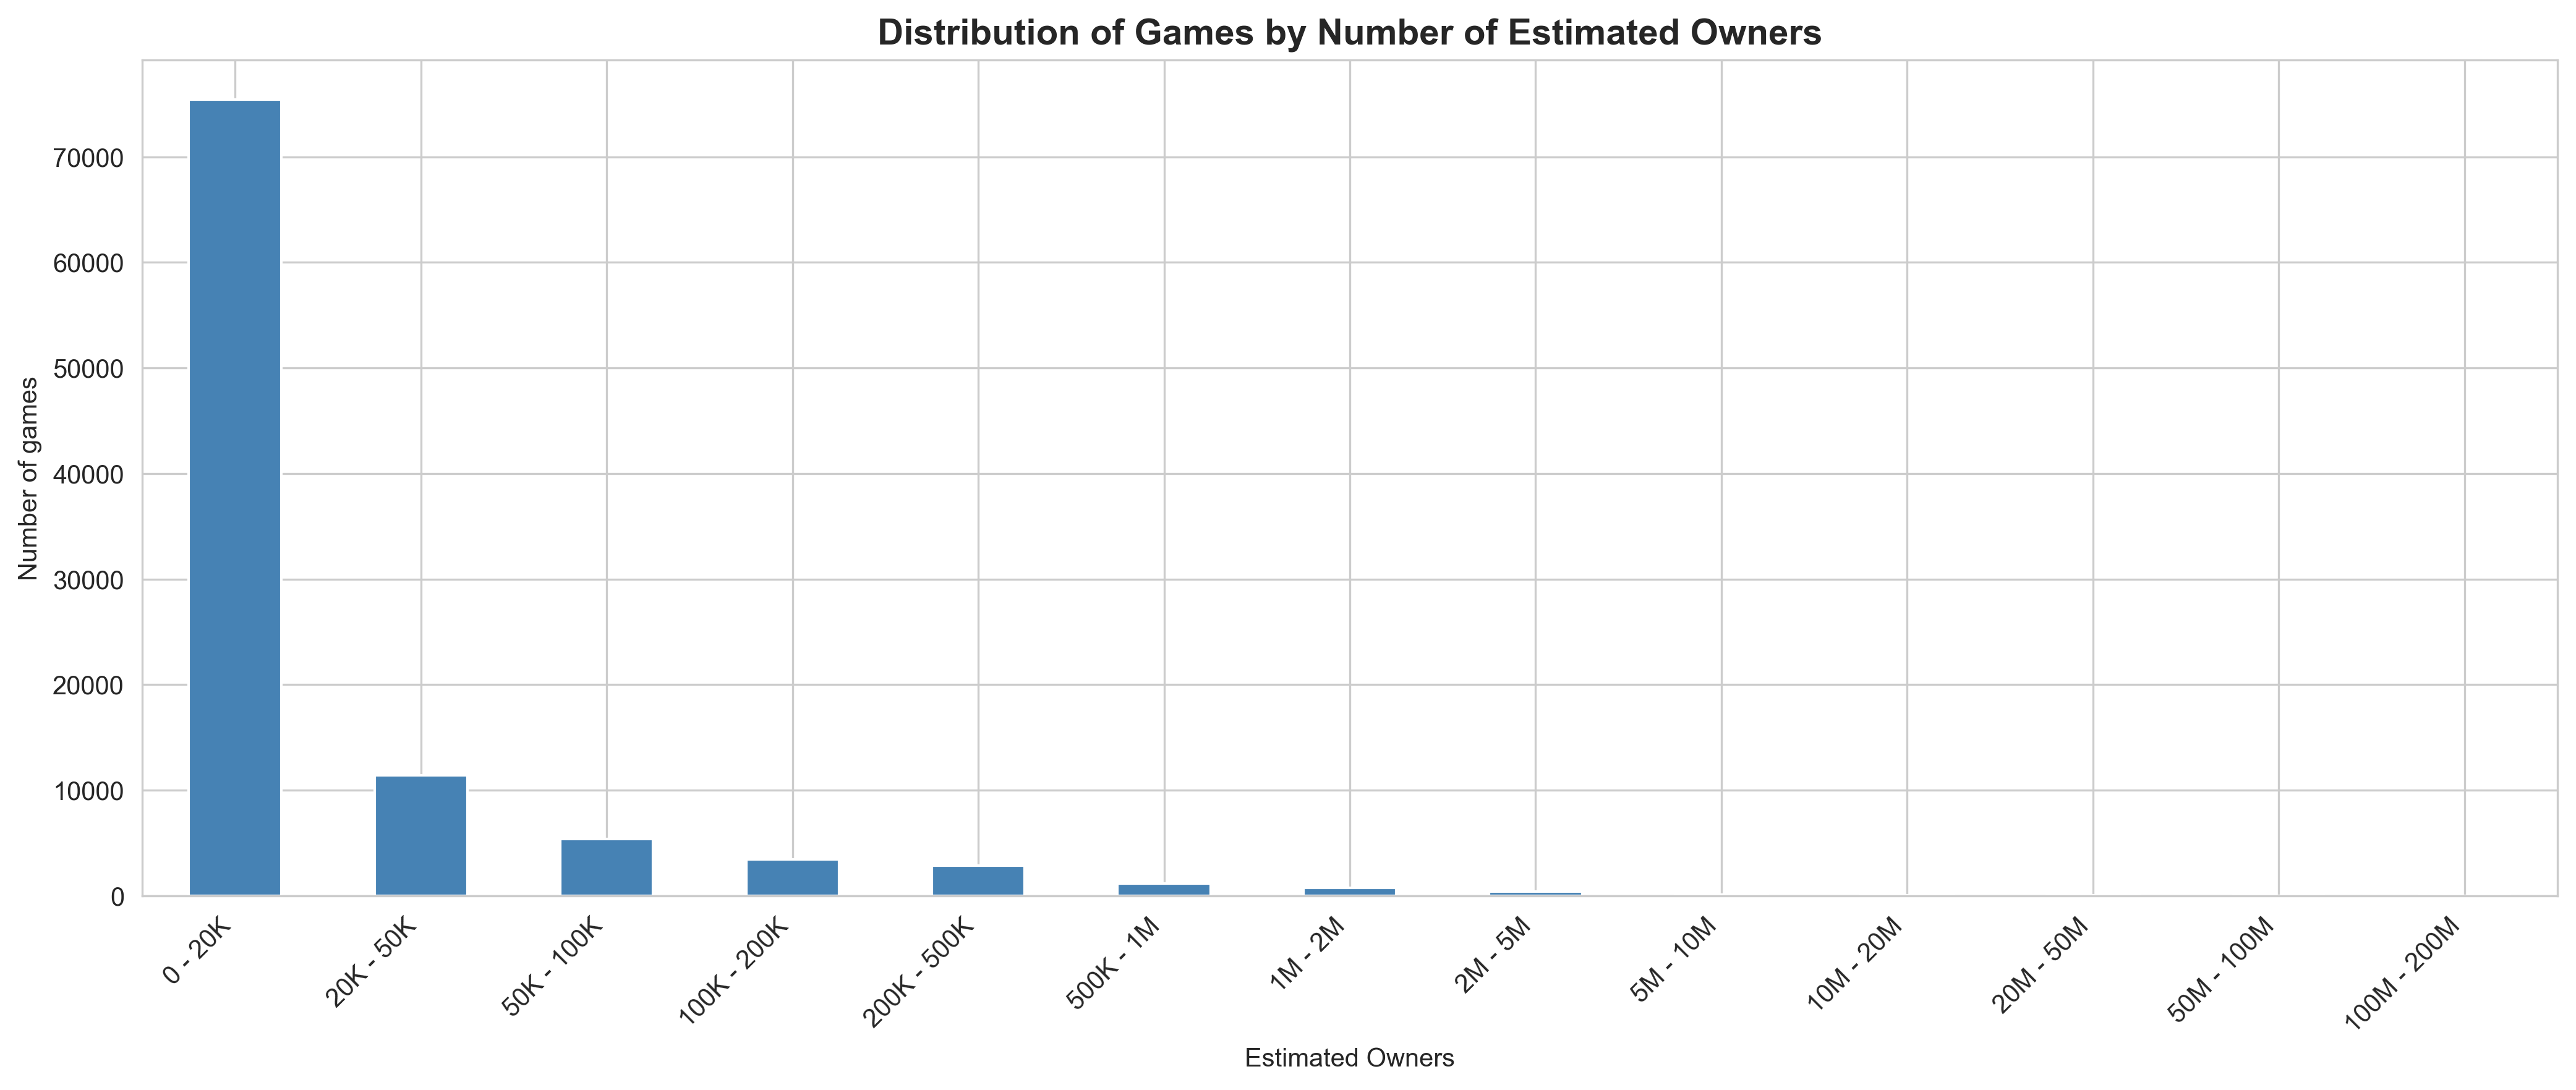
\includegraphics[width=0.8\linewidth]{Images/01_games_distribution.png}
    \caption{Phân phối số lượng game theo ước tính số lượng người sở hữu.}
    \label{fig:01_distribution}
\end{figure}
\hspace{1cm} Biểu đồ Hình \ref{fig:01_distribution} phản ánh một sự chênh lệch khổng lồ trong phân phối lượng người chơi. Một sự thật khắc nghiệt của ngành công nghiệp này là phần lớn các tựa game (hơn 75.000 trò chơi) chỉ quanh quẩn ở mức độ phổ biến rất thấp (0 - 20K người sở hữu). Càng tiến lên các cột mốc cao hơn (từ 50K đến hàng triệu), số lượng game càng giảm mạnh theo đường cong hàm mũ. Điều này cho thấy thị trường đang ở mức độ bão hòa cao, tỷ lệ đào thải cực kỳ khắc nghiệt. Việc lọt vào nhóm "game thành công" (được định nghĩa là trên 200K người sở hữu) đòi hỏi tựa game không chỉ tốt về mặt kỹ thuật mà còn phải có điểm nhấn mạnh mẽ trên thị trường.

\subsection{Chiến lược định giá: Sức mạnh của mô hình Free-to-Play}
\begin{figure}[ht]
    \centering
    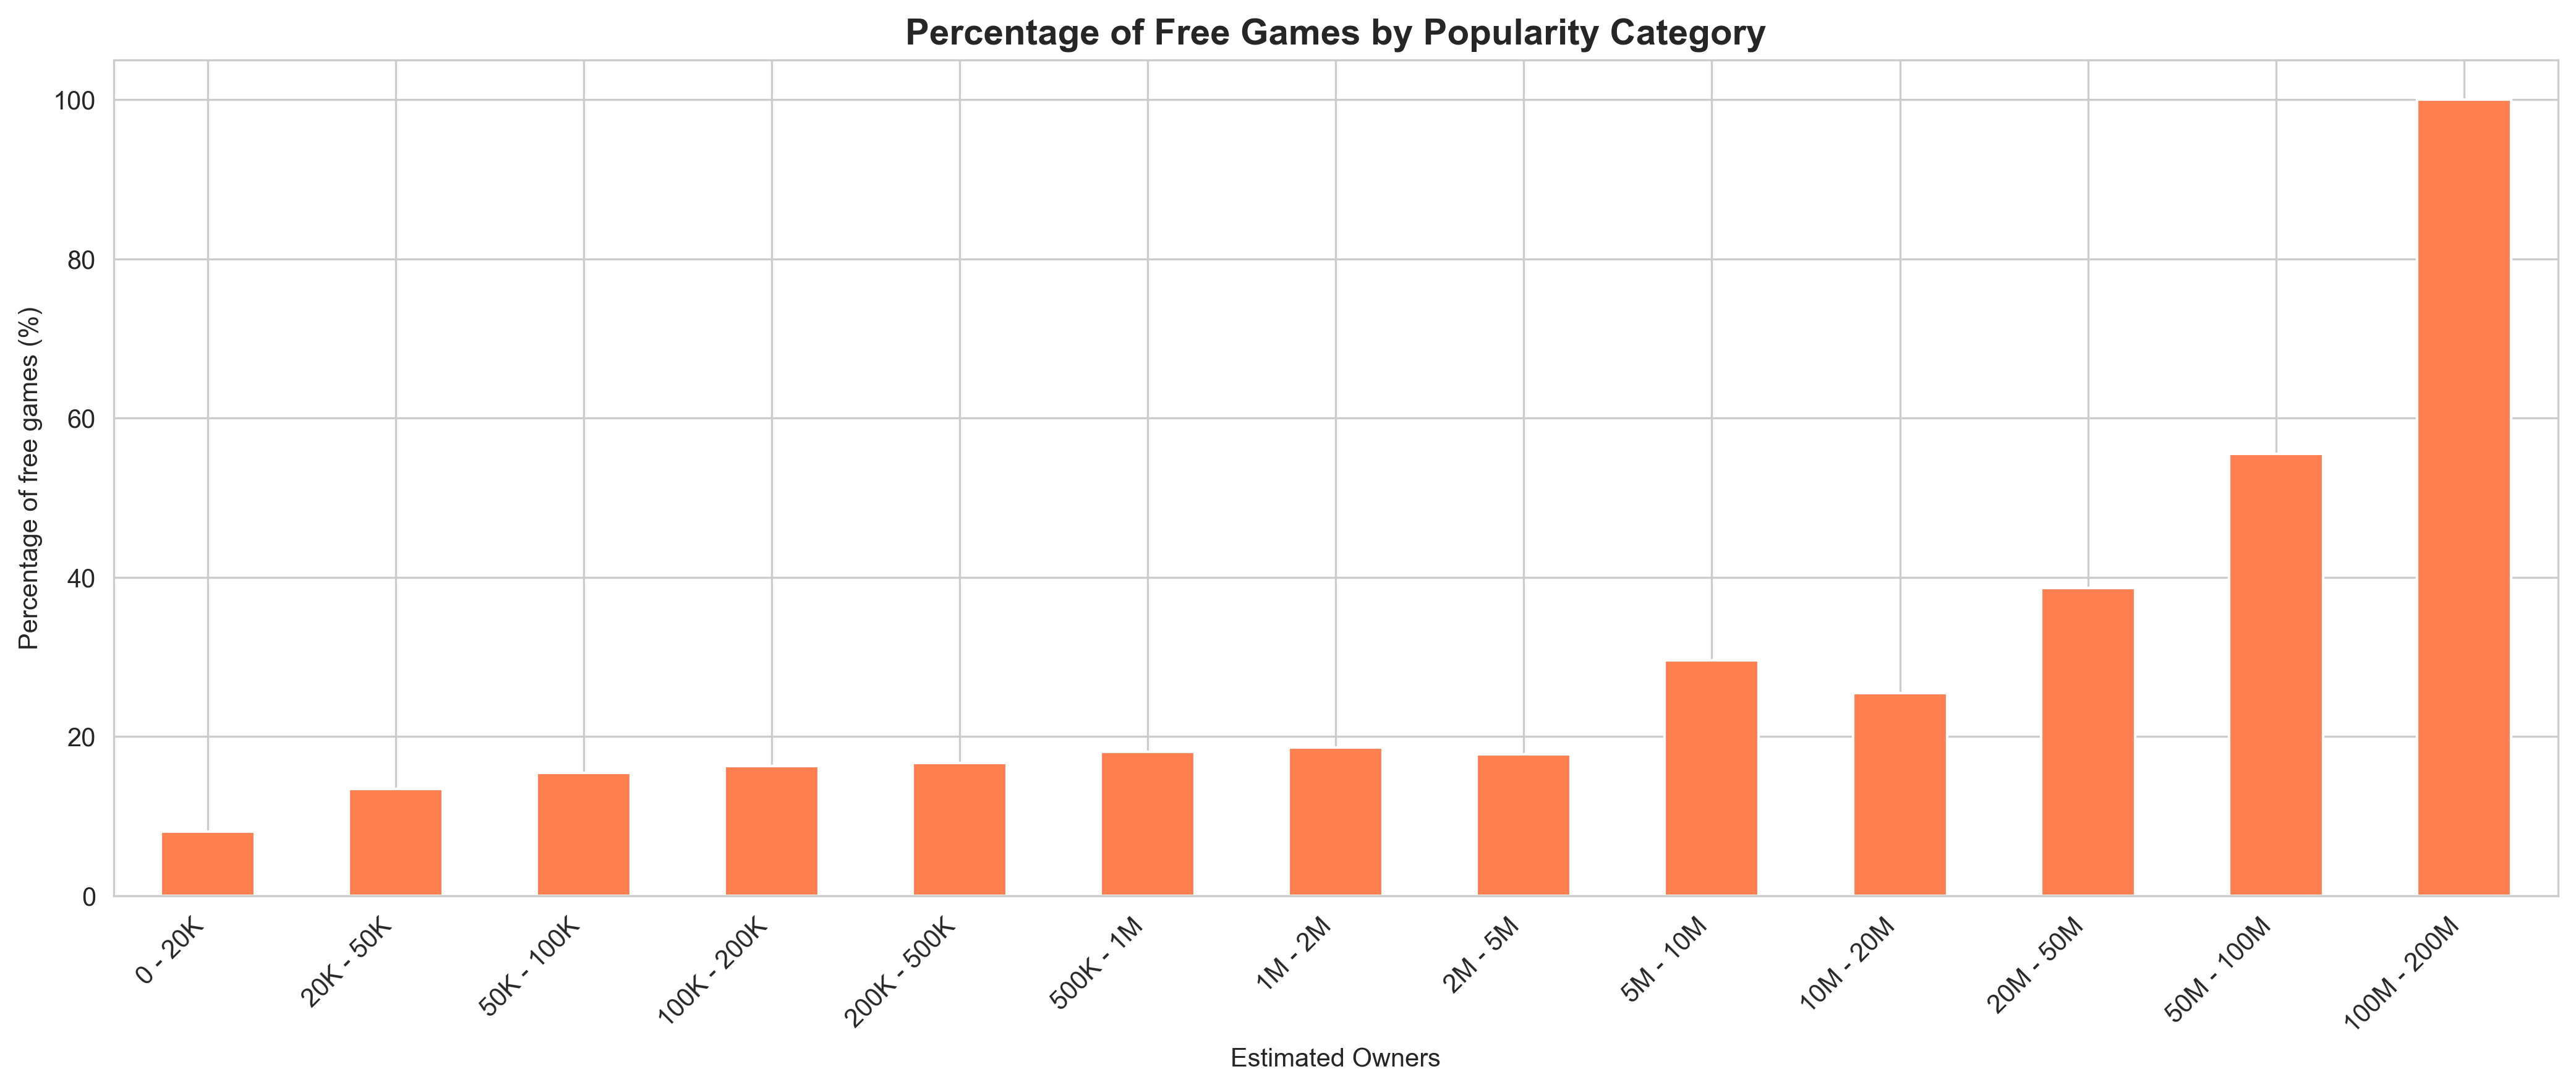
\includegraphics[width=0.48\linewidth]{Images/02_free_games_percentage.png}
    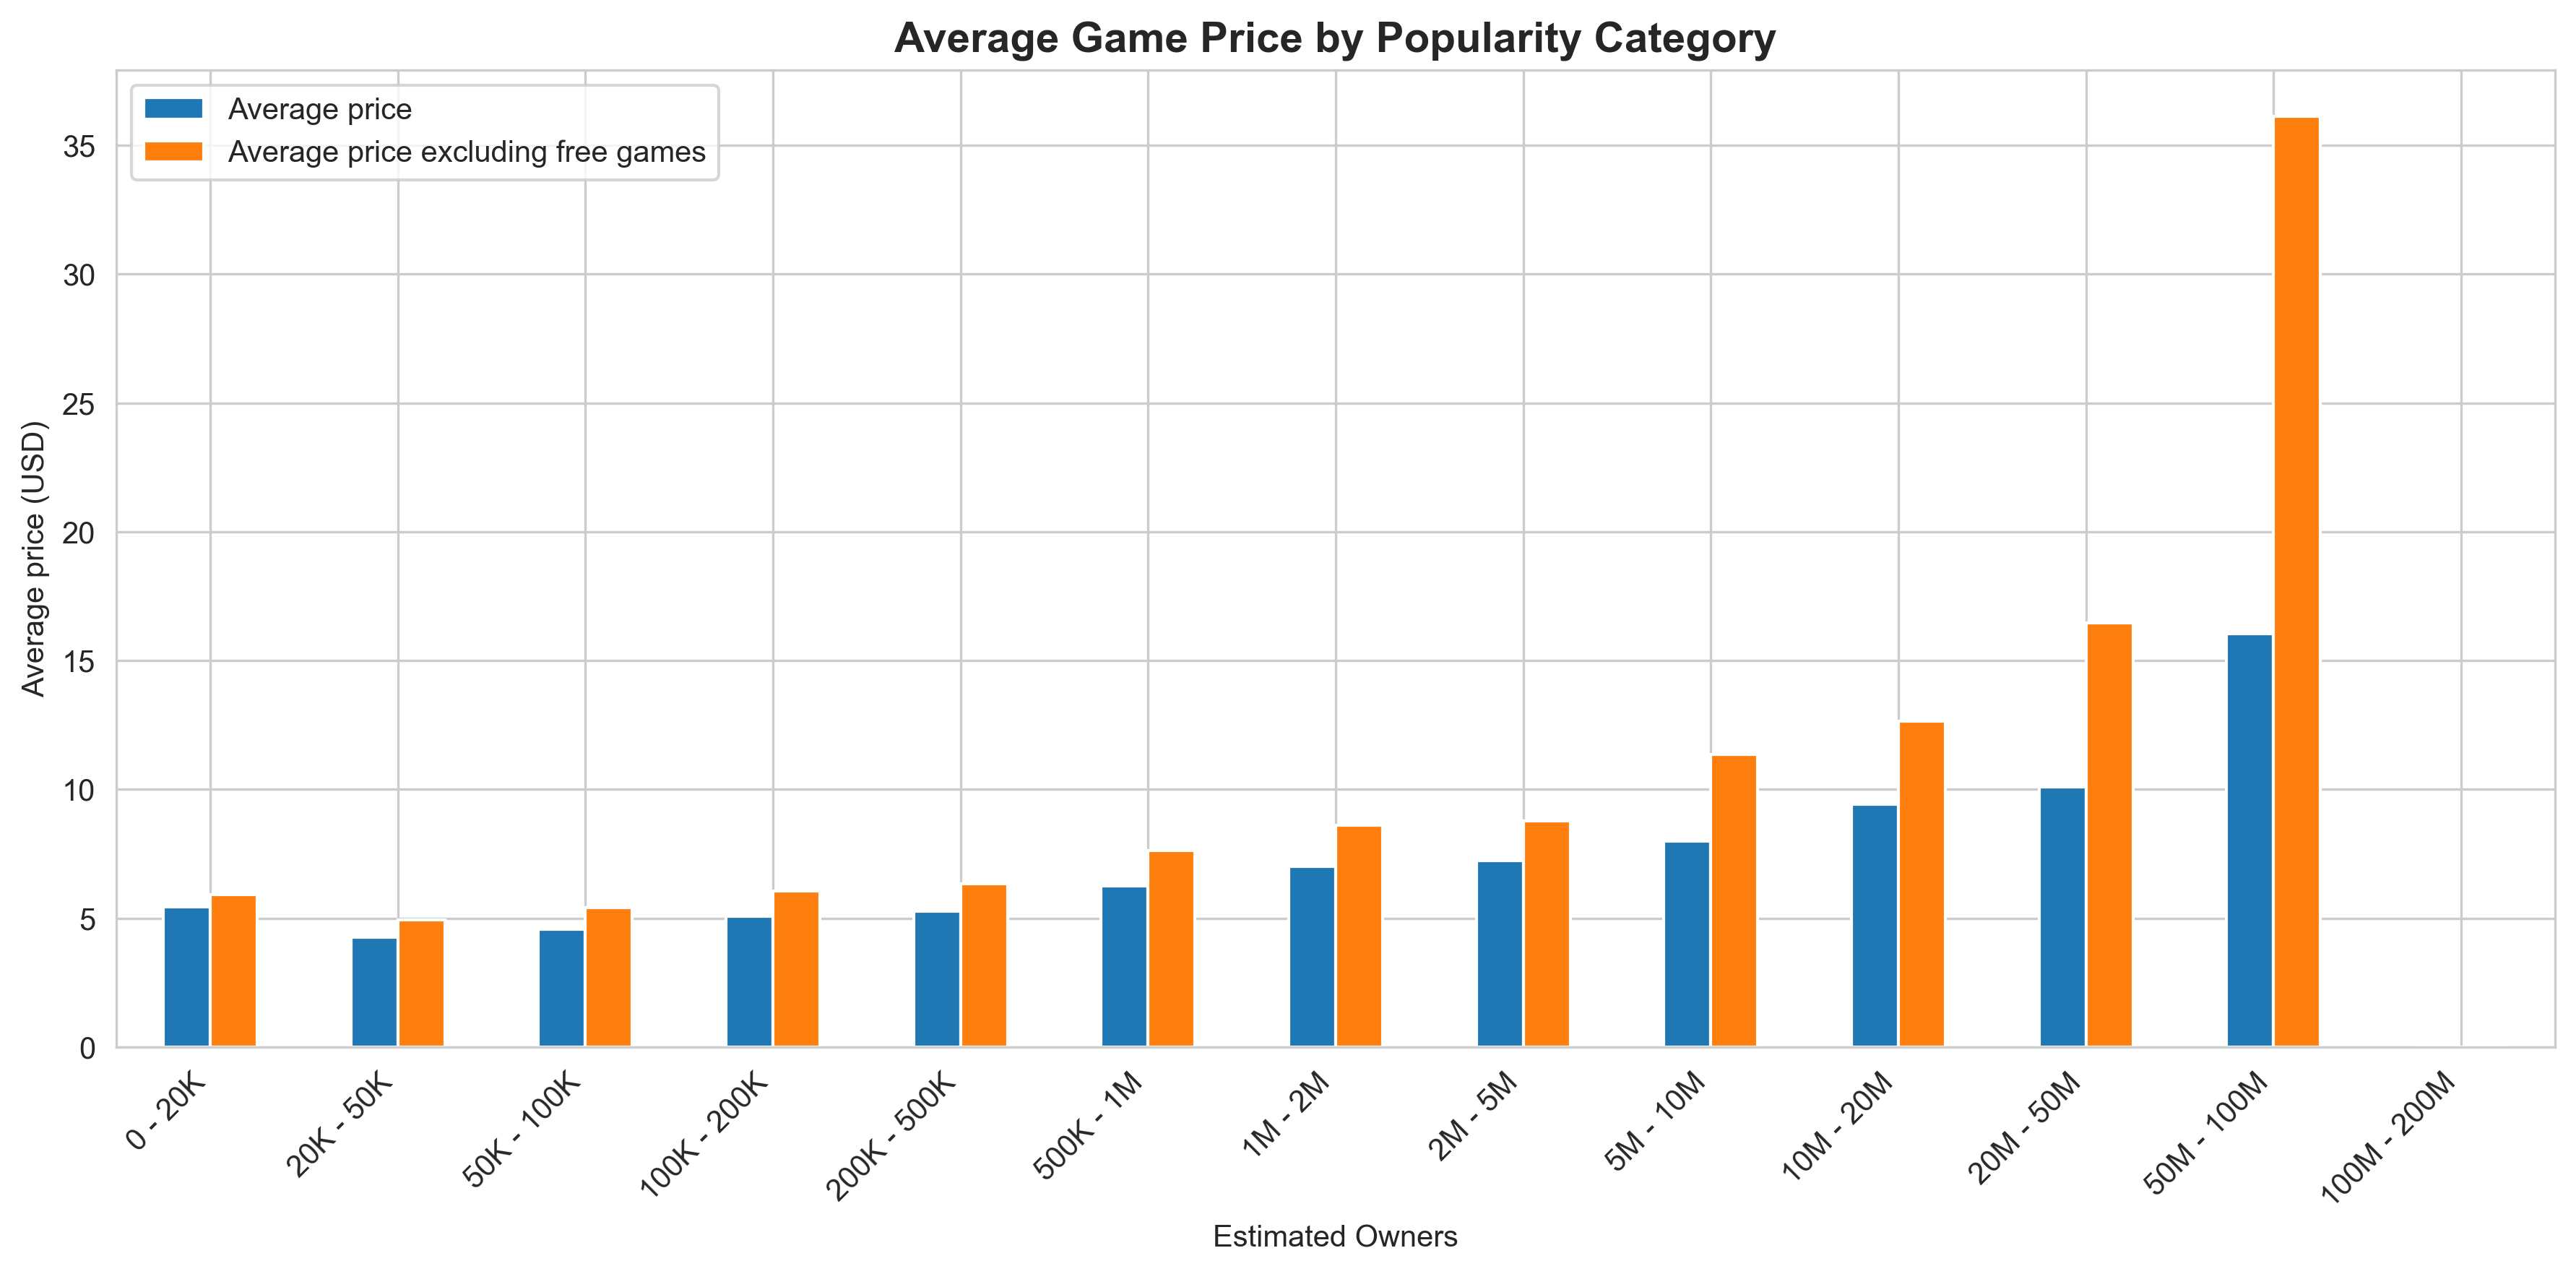
\includegraphics[width=0.48\linewidth]{Images/03_average_price.png}
    \caption{Tỷ lệ game miễn phí (trái) và Mức giá trung bình (phải) theo phân khúc phổ biến.}
    \label{fig:price_analysis}
\end{figure}
\hspace{1cm} Phân tích chiến lược định giá thông qua Hình \ref{fig:price_analysis} mang lại những góc nhìn có giá trị cao cho các nhà phát hành. Nhìn vào đồ thị bên trái, ta thấy mức độ phổ biến của game tỷ lệ thuận với khả năng tựa game đó là "Free-to-Play". Đặc biệt ở nhóm siêu phổ biến (100M - 200M người sở hữu), tỷ lệ game miễn phí đạt mức tuyệt đối 100\%. Điều này khẳng định sức mạnh vô song của mô hình kinh doanh dựa trên vi giao dịch (microtransactions) và bán vật phẩm ảo (in-game items) trong việc thu hút hàng triệu người chơi ban đầu.\\

\hspace{1cm} Tuy nhiên, đối với các tựa game trả phí (đồ thị bên phải, cột màu cam), giá bán trung bình lại có xu hướng tăng dần ở các phân khúc người chơi cao hơn (như nhóm 20M-50M và 50M-100M). Phân tích này tiết lộ một tâm lý tiêu dùng: người chơi hoàn toàn sẵn sàng chi trả một số tiền lớn (từ 15\$ đến hơn 35\$) nếu tựa game đó thực sự là một bom tấn (AAA) chất lượng, xứng đáng với giá tiền.

\subsection{Chất lượng sản phẩm qua lăng kính đánh giá (Reviews)}
\begin{figure}[ht]
    \centering
    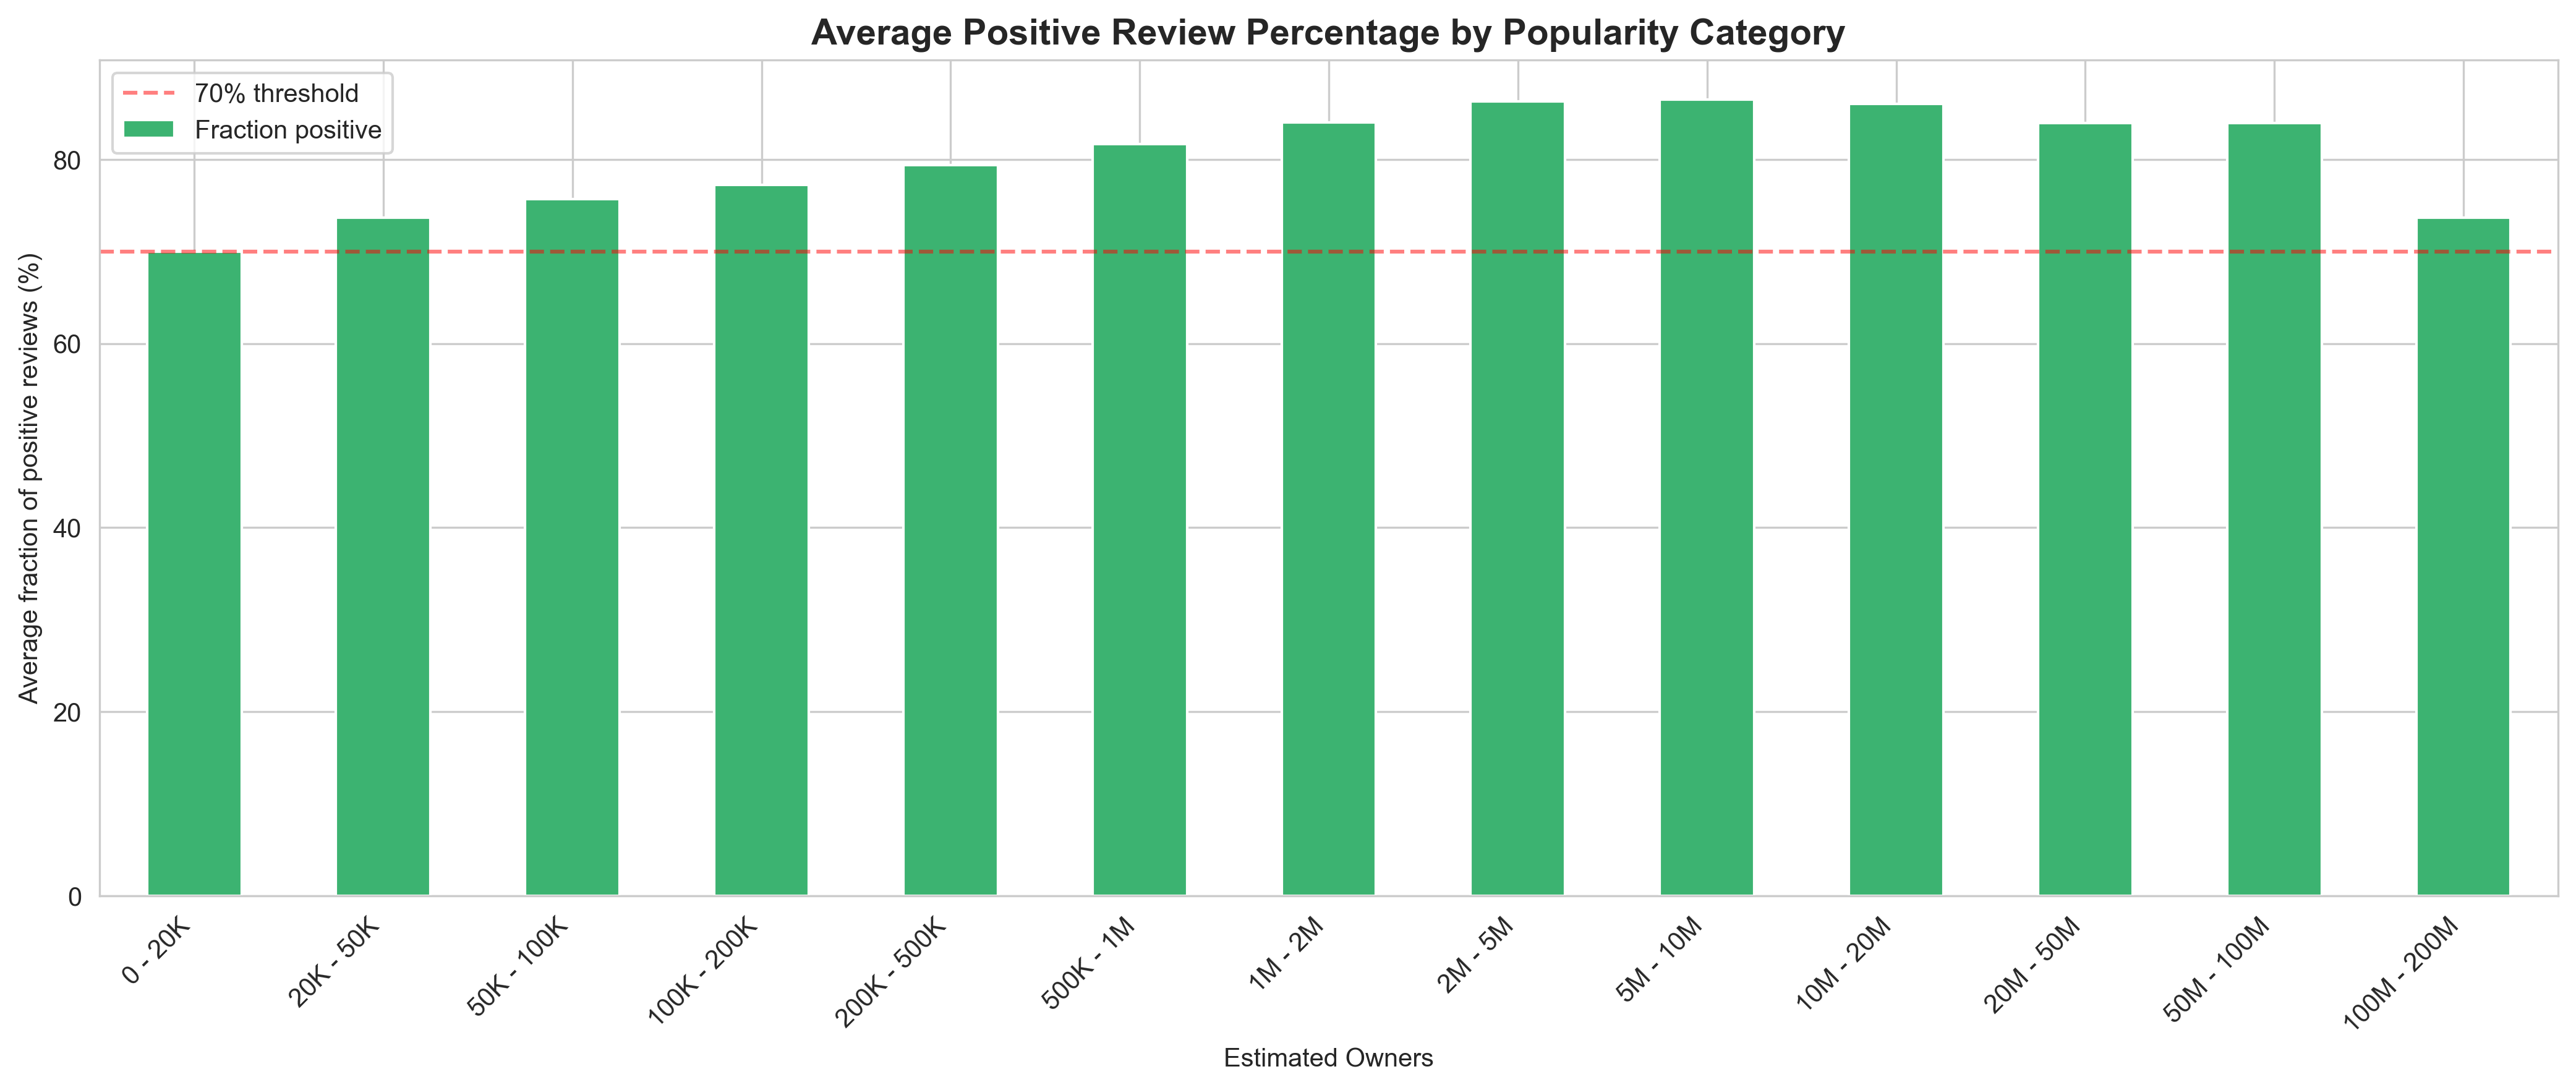
\includegraphics[width=0.8\linewidth]{Images/04_positive_reviews.png}
    \caption{Tỷ lệ đánh giá tích cực trung bình theo phân khúc người chơi.}
    \label{fig:04_reviews}
\end{figure}
\hspace{1cm} Đánh giá từ cộng đồng (User Reviews) là thước đo sinh tồn kéo dài vòng đời của mọi trò chơi điện tử. Đồ thị Hình \ref{fig:04_reviews} cho thấy một quy luật đồng nhất: tất cả các nhóm game từ mức 20K người sở hữu trở lên đều có tỷ lệ đánh giá tích cực trung bình vượt qua ngưỡng an toàn 70\%. Đáng chú ý, các nhóm game cực kỳ phổ biến (từ 500K đến 100M) luôn duy trì mức đánh giá trên 80\%. Điều này tái khẳng định rằng truyền miệng là công cụ marketing mạnh nhất; một tựa game không thể lan truyền và giữ chân cộng đồng lớn nếu bản thân nó chứa đầy lỗi (bugs) hoặc có thiết kế kém.

\subsection{Đầu tư hình ảnh thương hiệu và nền tảng kỹ thuật}
\begin{figure}[ht]
    \centering
    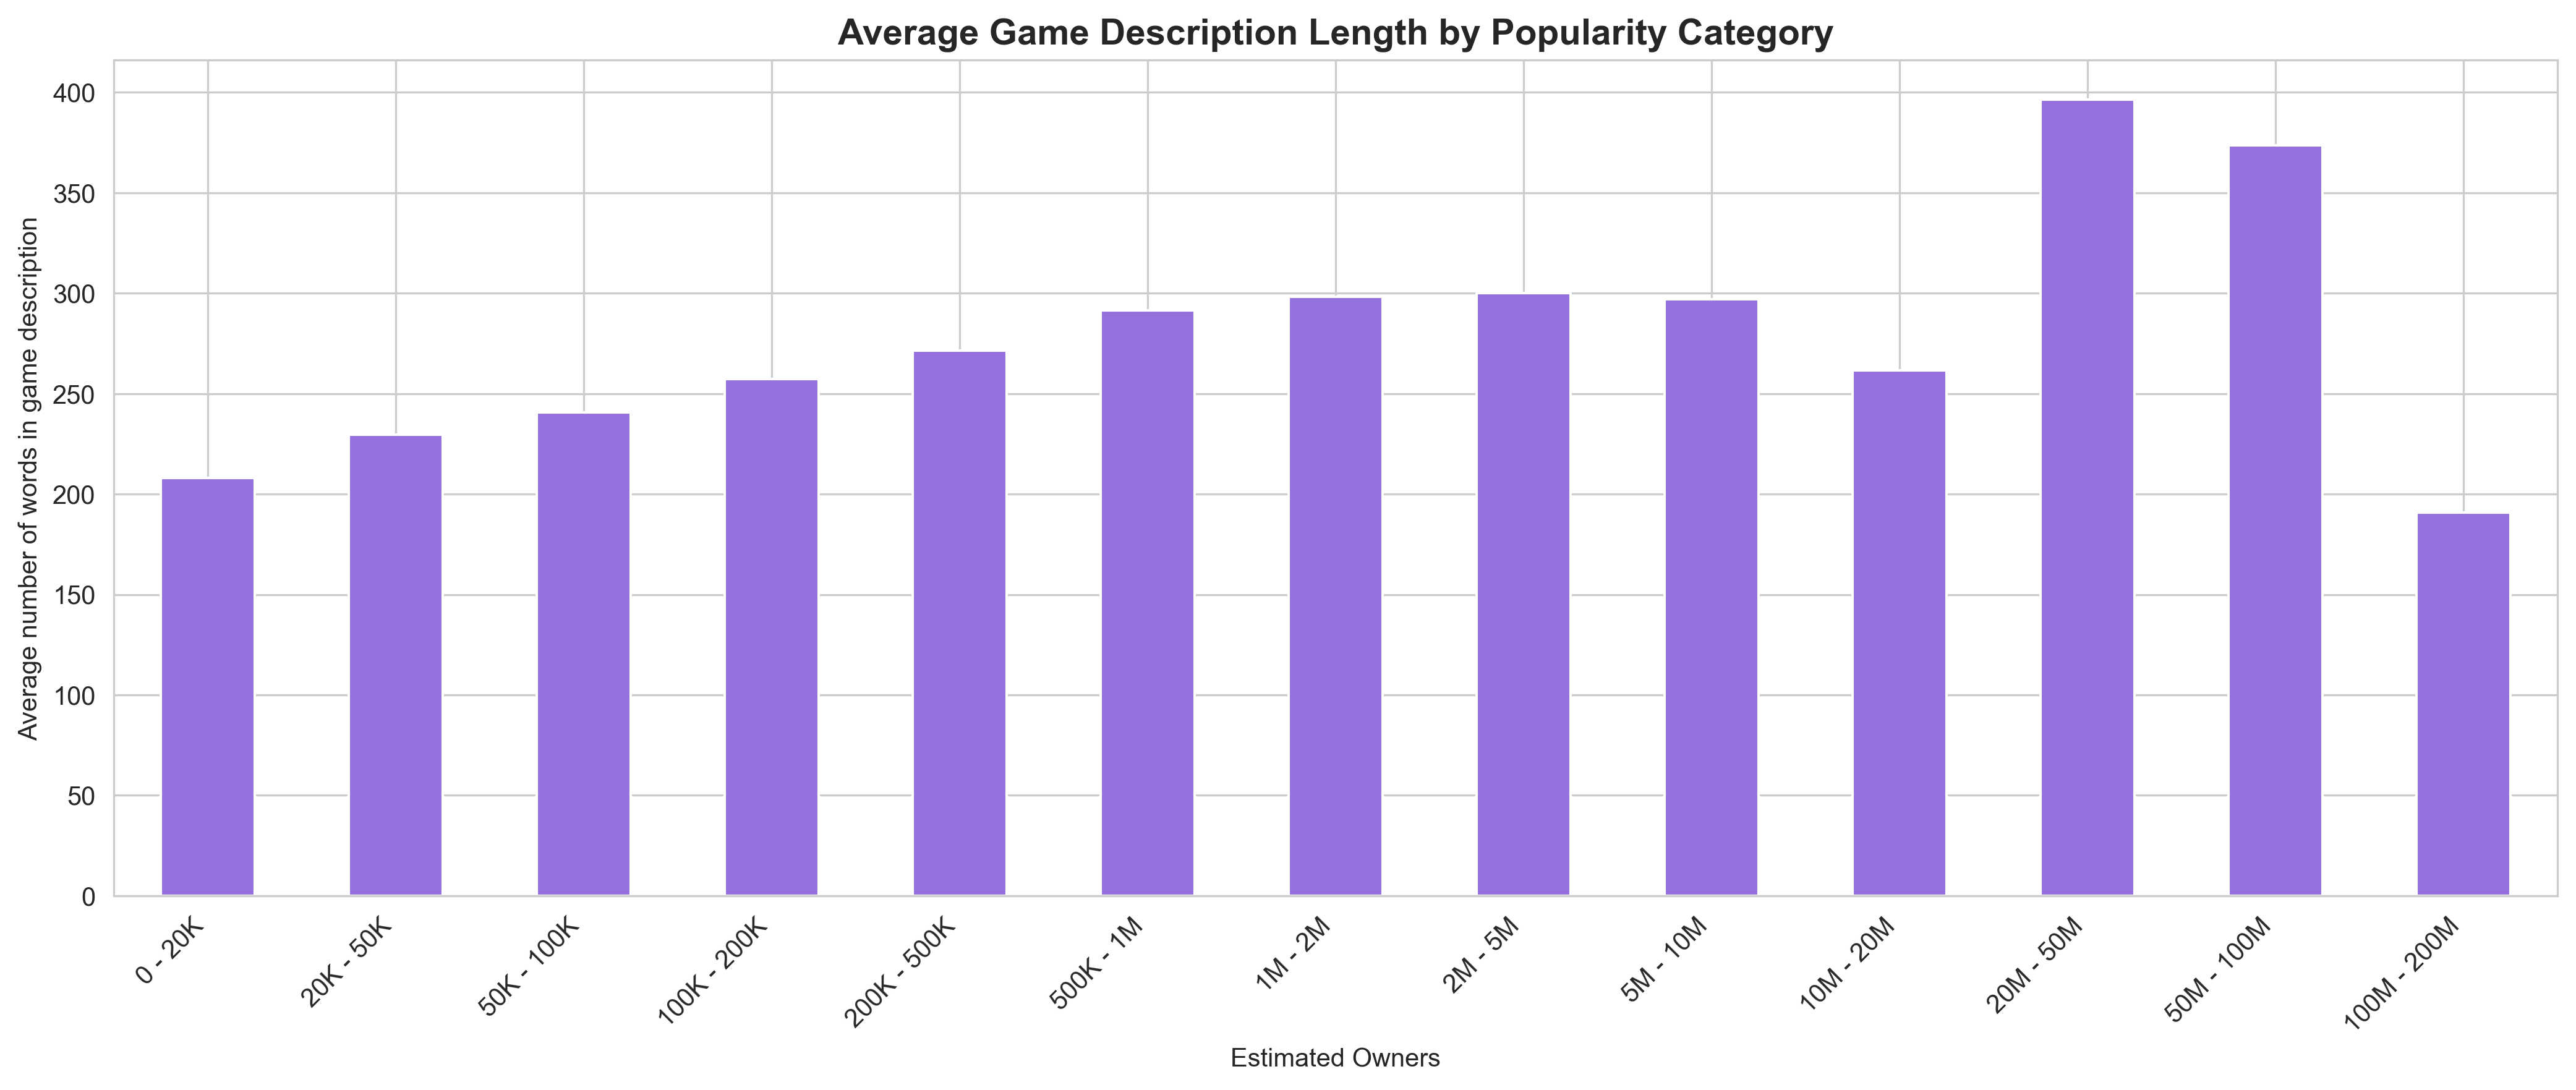
\includegraphics[width=0.48\linewidth]{Images/06_description_length.png}
    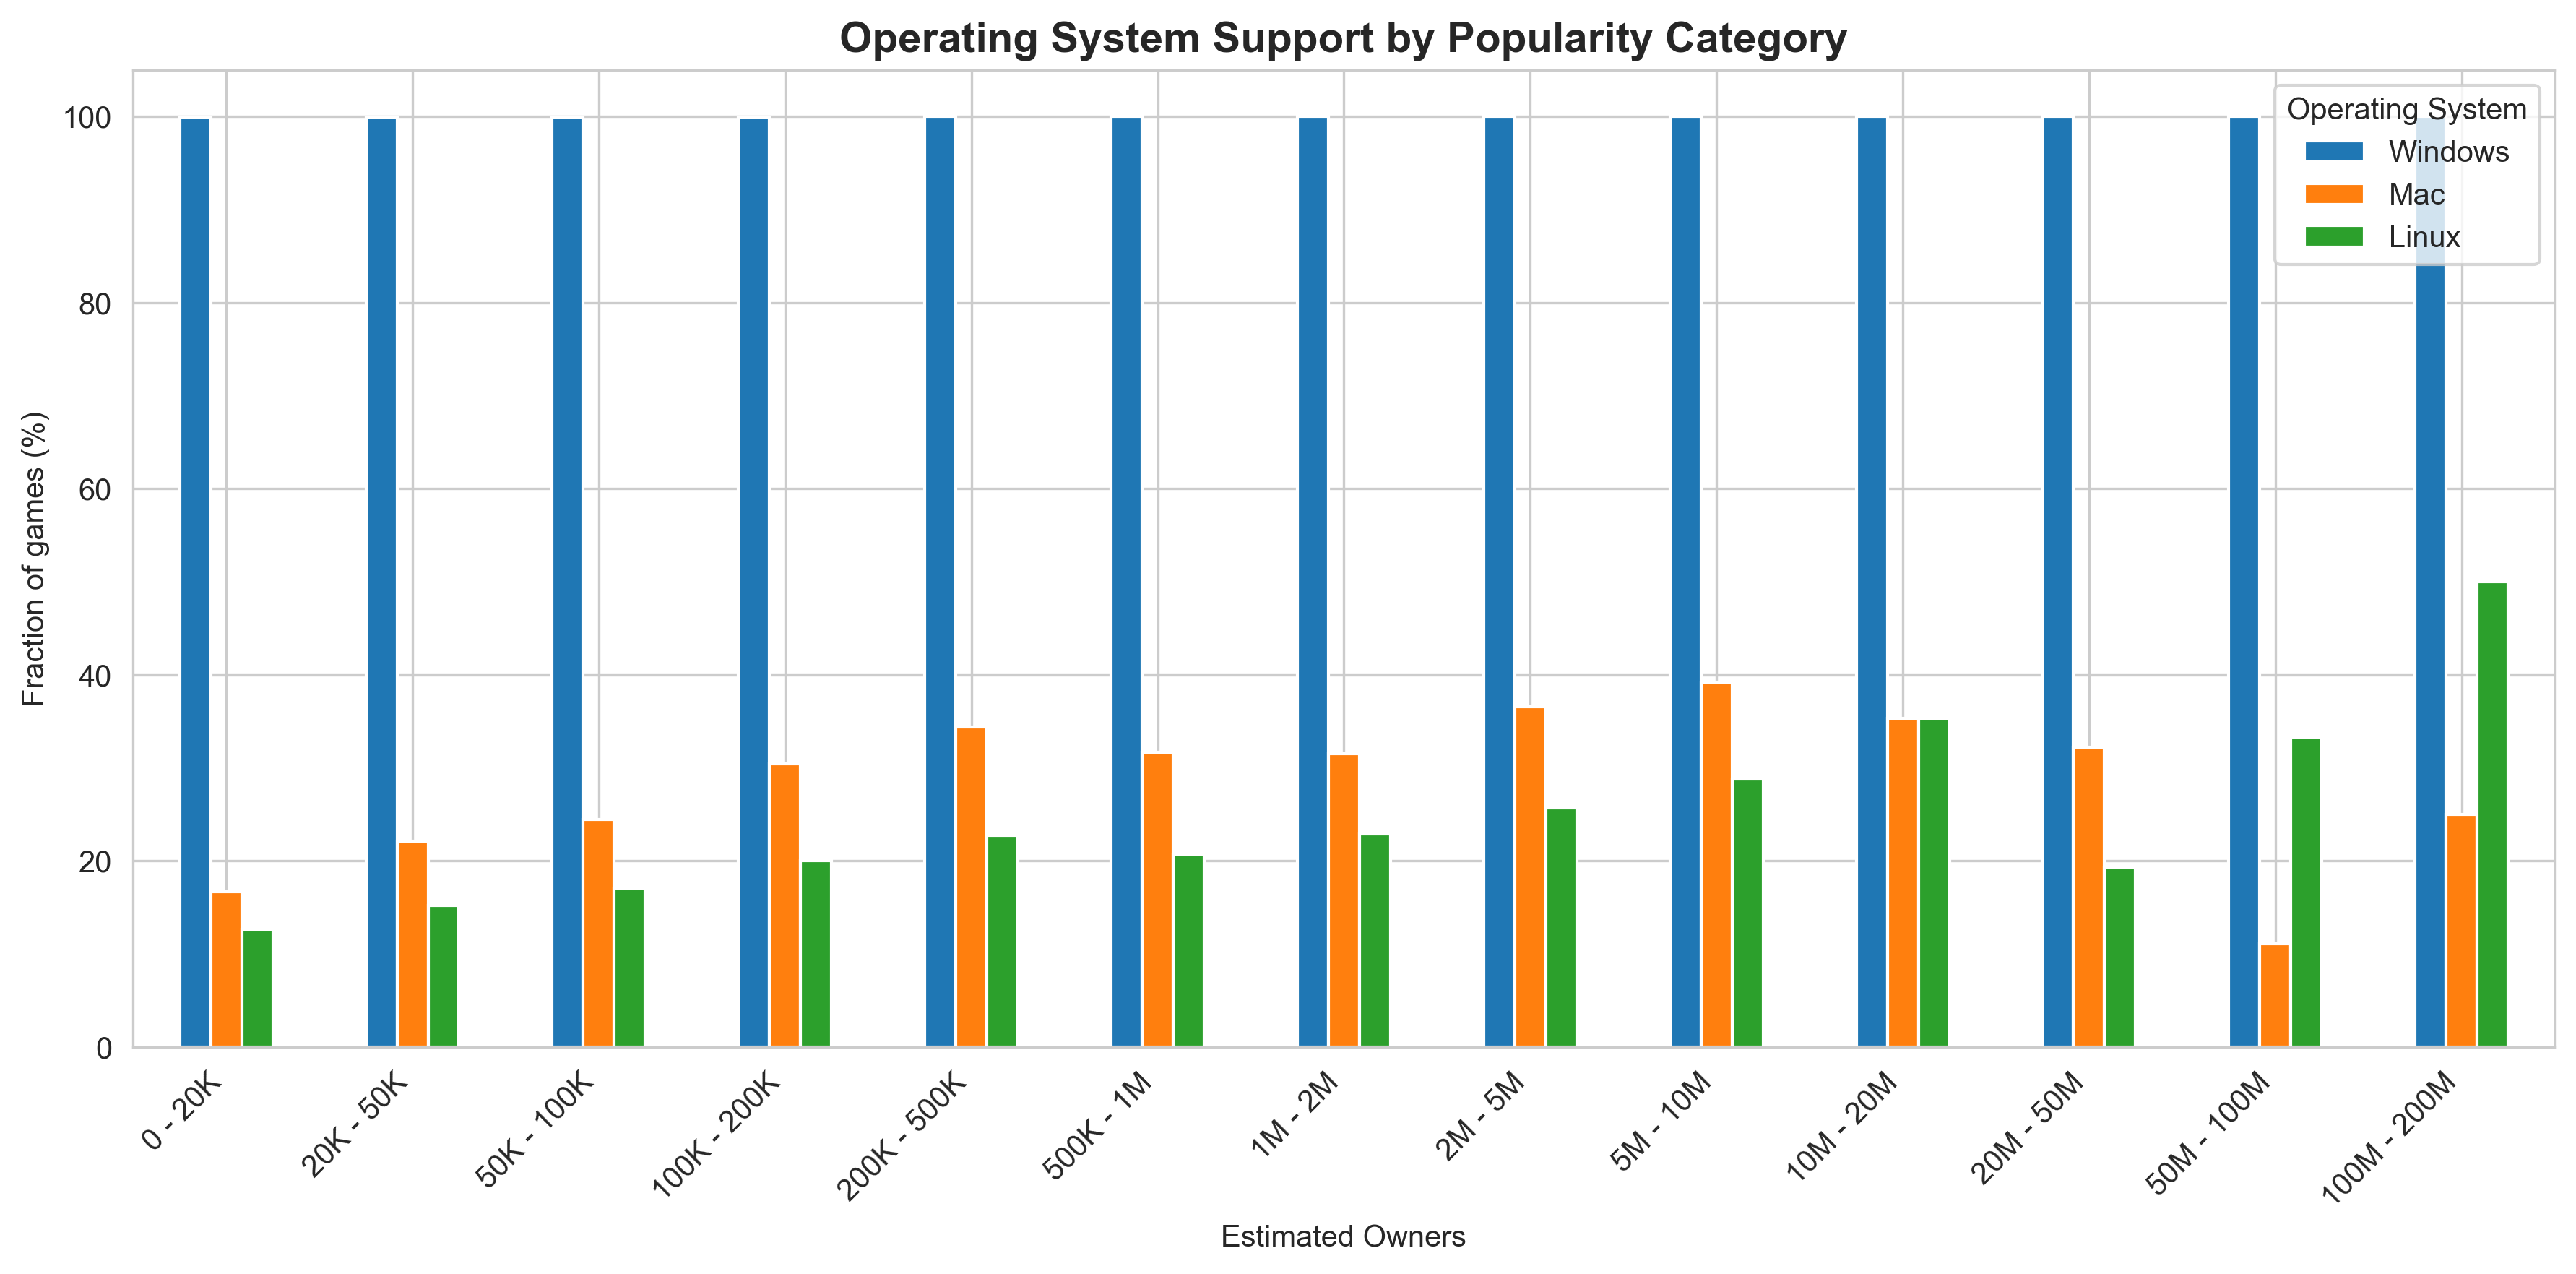
\includegraphics[width=0.48\linewidth]{Images/07_os_support.png}
    \caption{Chiều dài mô tả game (trái) và Tỷ lệ hỗ trợ hệ điều hành (phải).}
    \label{fig:desc_os}
\end{figure}
\hspace{1cm} Về khía cạnh thương hiệu (Hình \ref{fig:desc_os} trái), độ dài mô tả game thể hiện sự chăm chút của nhà phát hành. Các tựa game càng thành công thì nhà phát triển càng đầu tư viết mô tả chi tiết, cốt truyện rõ ràng (đạt trung bình từ 300 đến 400 từ). Ngoại lệ duy nhất nằm ở nhóm 100M-200M, nơi các tựa game đã định hình thương hiệu quá mạnh (như Dota 2, CS:GO) nên không cần giải thích quá dài dòng.
\\

\hspace{1cm} Về nền tảng kỹ thuật (Hình \ref{fig:desc_os} phải), trong khi Windows là nền tảng bắt buộc (chiếm tỷ lệ 100\%), ta có thể thấy mức độ hỗ trợ macOS và Linux (các cột màu cam và xanh lá) gia tăng rõ rệt ở các tập game thành công hơn. Việc bỏ công sức biên dịch (port) game sang đa nền tảng giúp khai thác tối đa mọi ngách của thị trường.

\subsection{Xu hướng thể loại game (Genres) qua không gian và thời gian}
\begin{figure}[H]
    \centering
    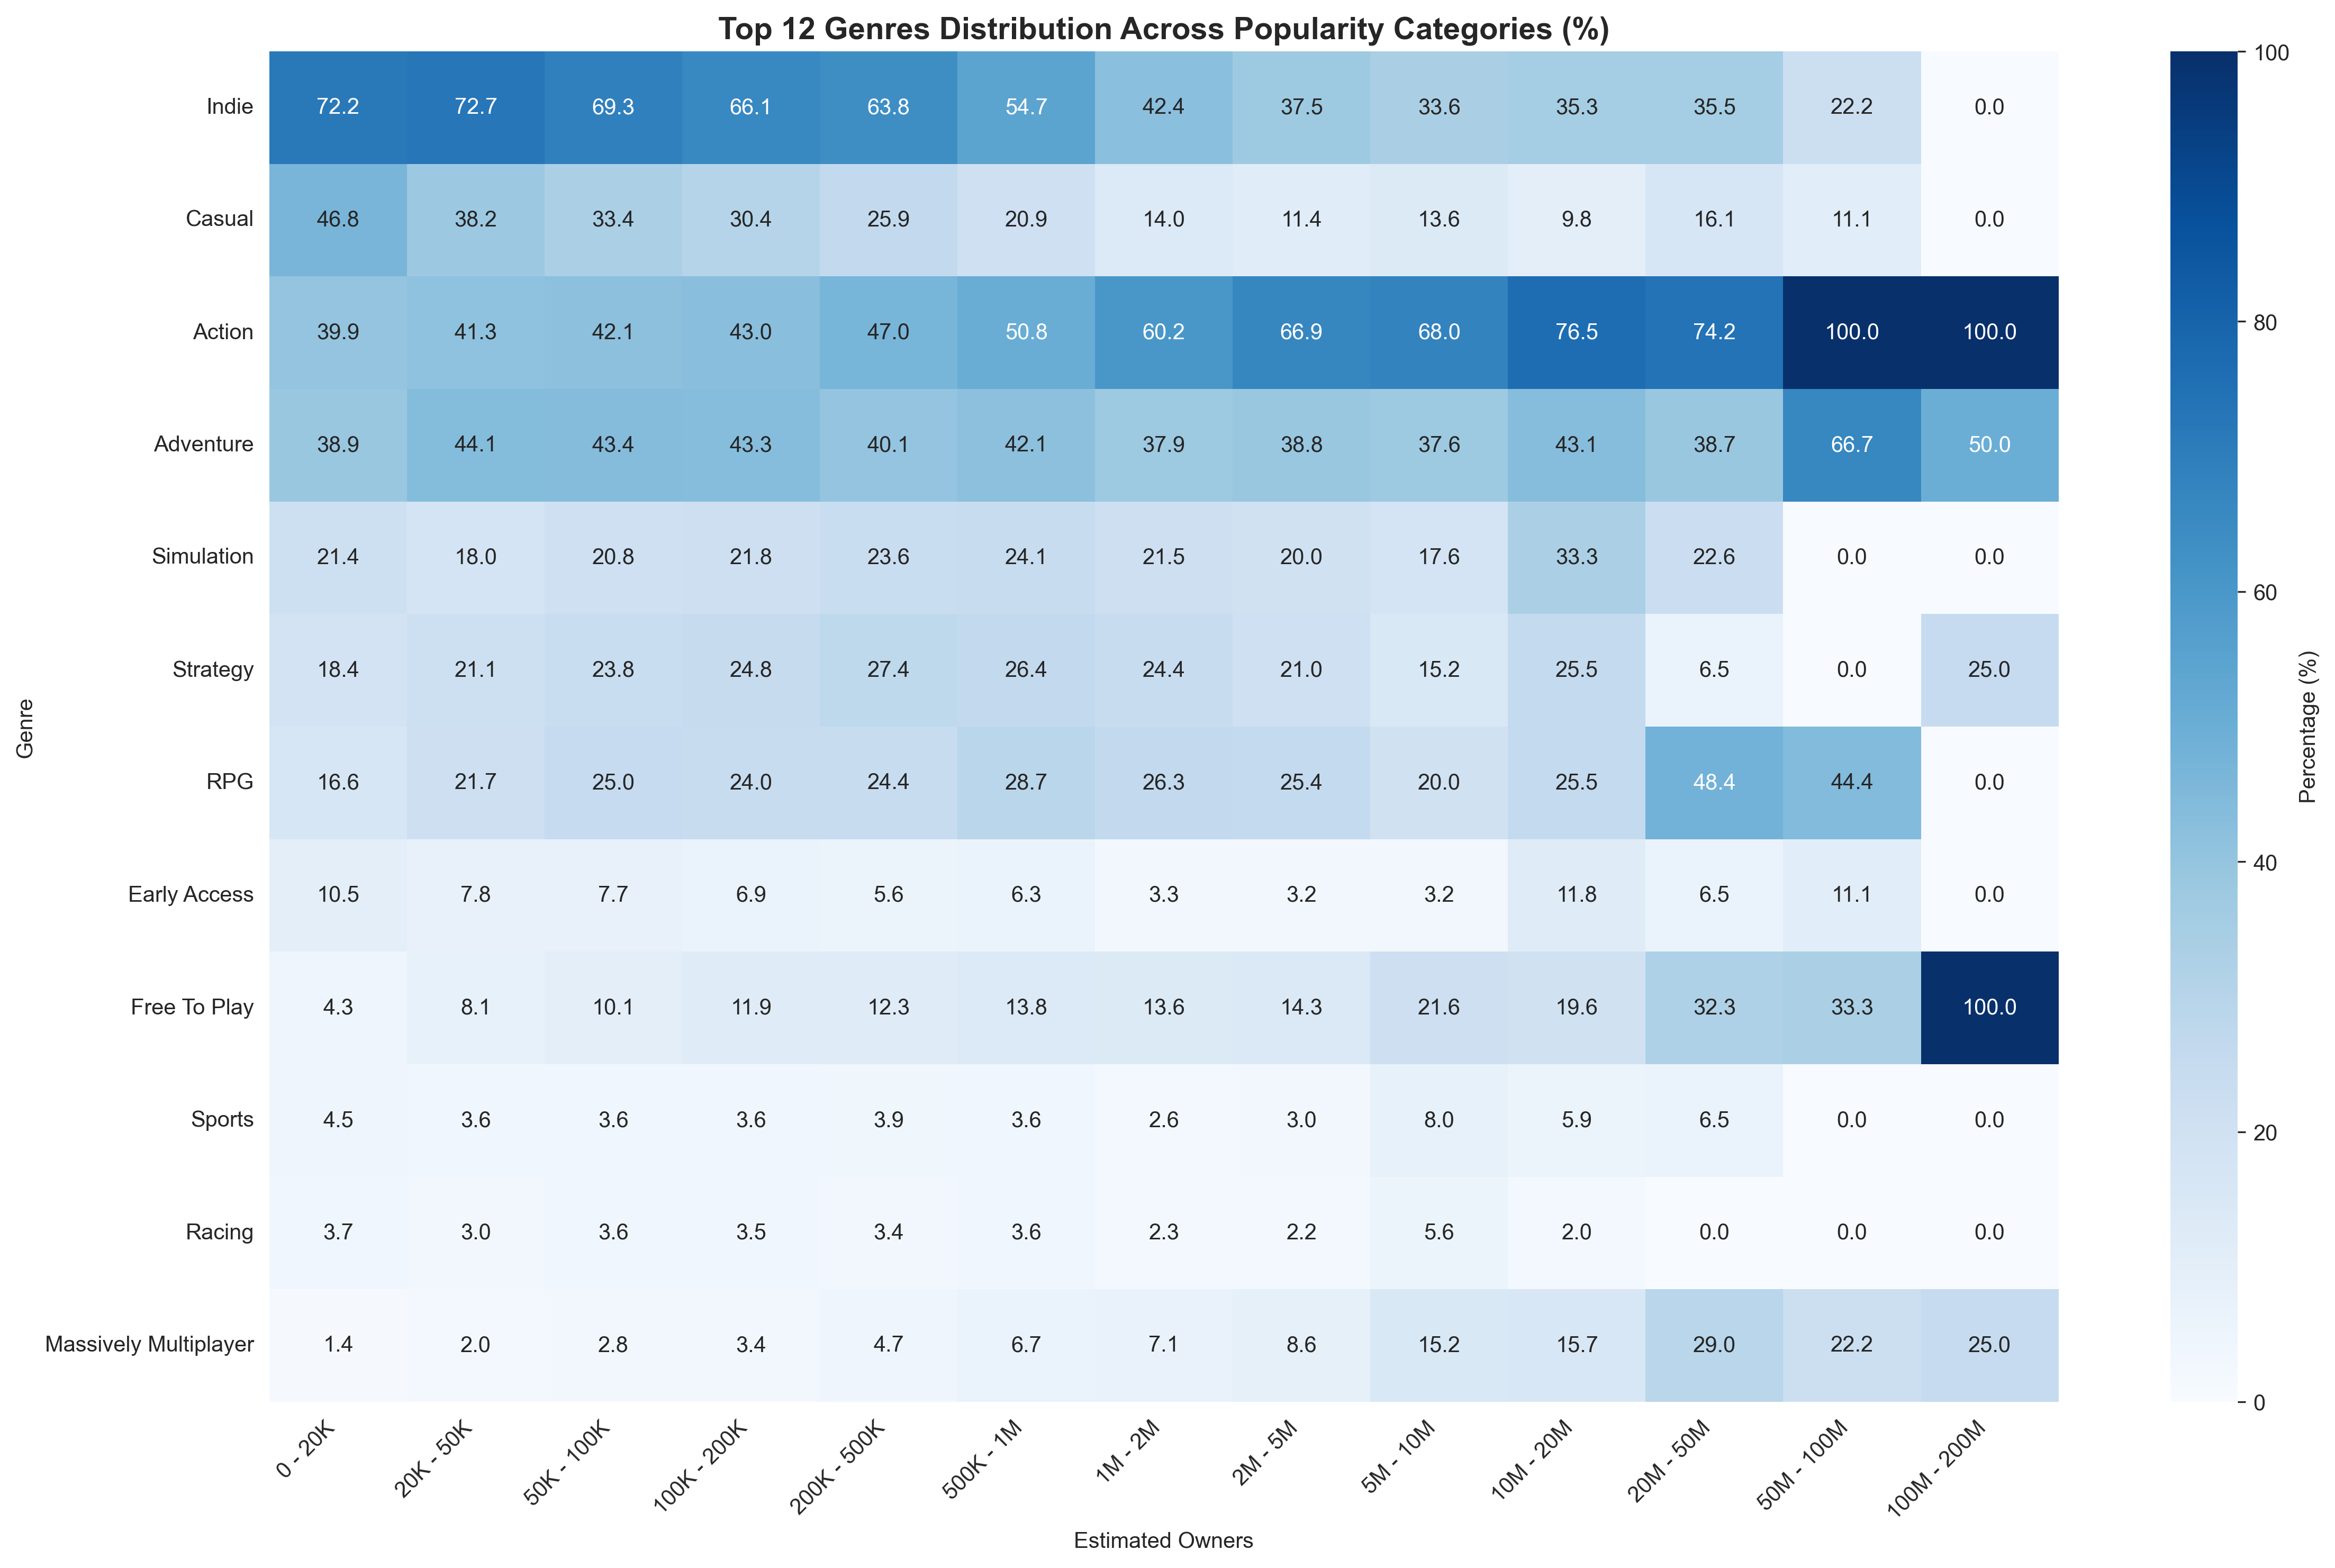
\includegraphics[width=0.8\linewidth]{Images/05_genre_heatmap.png}
    \caption{Bản đồ nhiệt phân bố Top 12 thể loại theo mức độ phổ biến.}
    \label{fig:05_genre_heatmap}
\end{figure}
\hspace{1cm} Quan sát bản đồ nhiệt phân phối thể loại (Hình \ref{fig:05_genre_heatmap}), hai thể loại "Action" và "Adventure" luôn giữ nhịp độ ổn định, chiếm tỷ trọng rất cao ở mọi phân khúc phổ biến. Đặc biệt, đúng như phân tích về giá ở trên, nhãn "Free to Play" tập trung cực kỳ đậm đặc ở cột phân khúc 100M-200M (chiếm 100\%). Một điểm thú vị khác là thể loại "Indie" thống trị thị phần ở các phân khúc người chơi thấp và trung bình (0 - 1M) nhưng lại hoàn toàn biến mất ở phân khúc vĩ đại (trên 50M), phản ánh "bức tường kính" về giới hạn ngân sách truyền thông của các studio độc lập so với các tập đoàn giải trí lớn.

\begin{figure}[H]
    \centering
    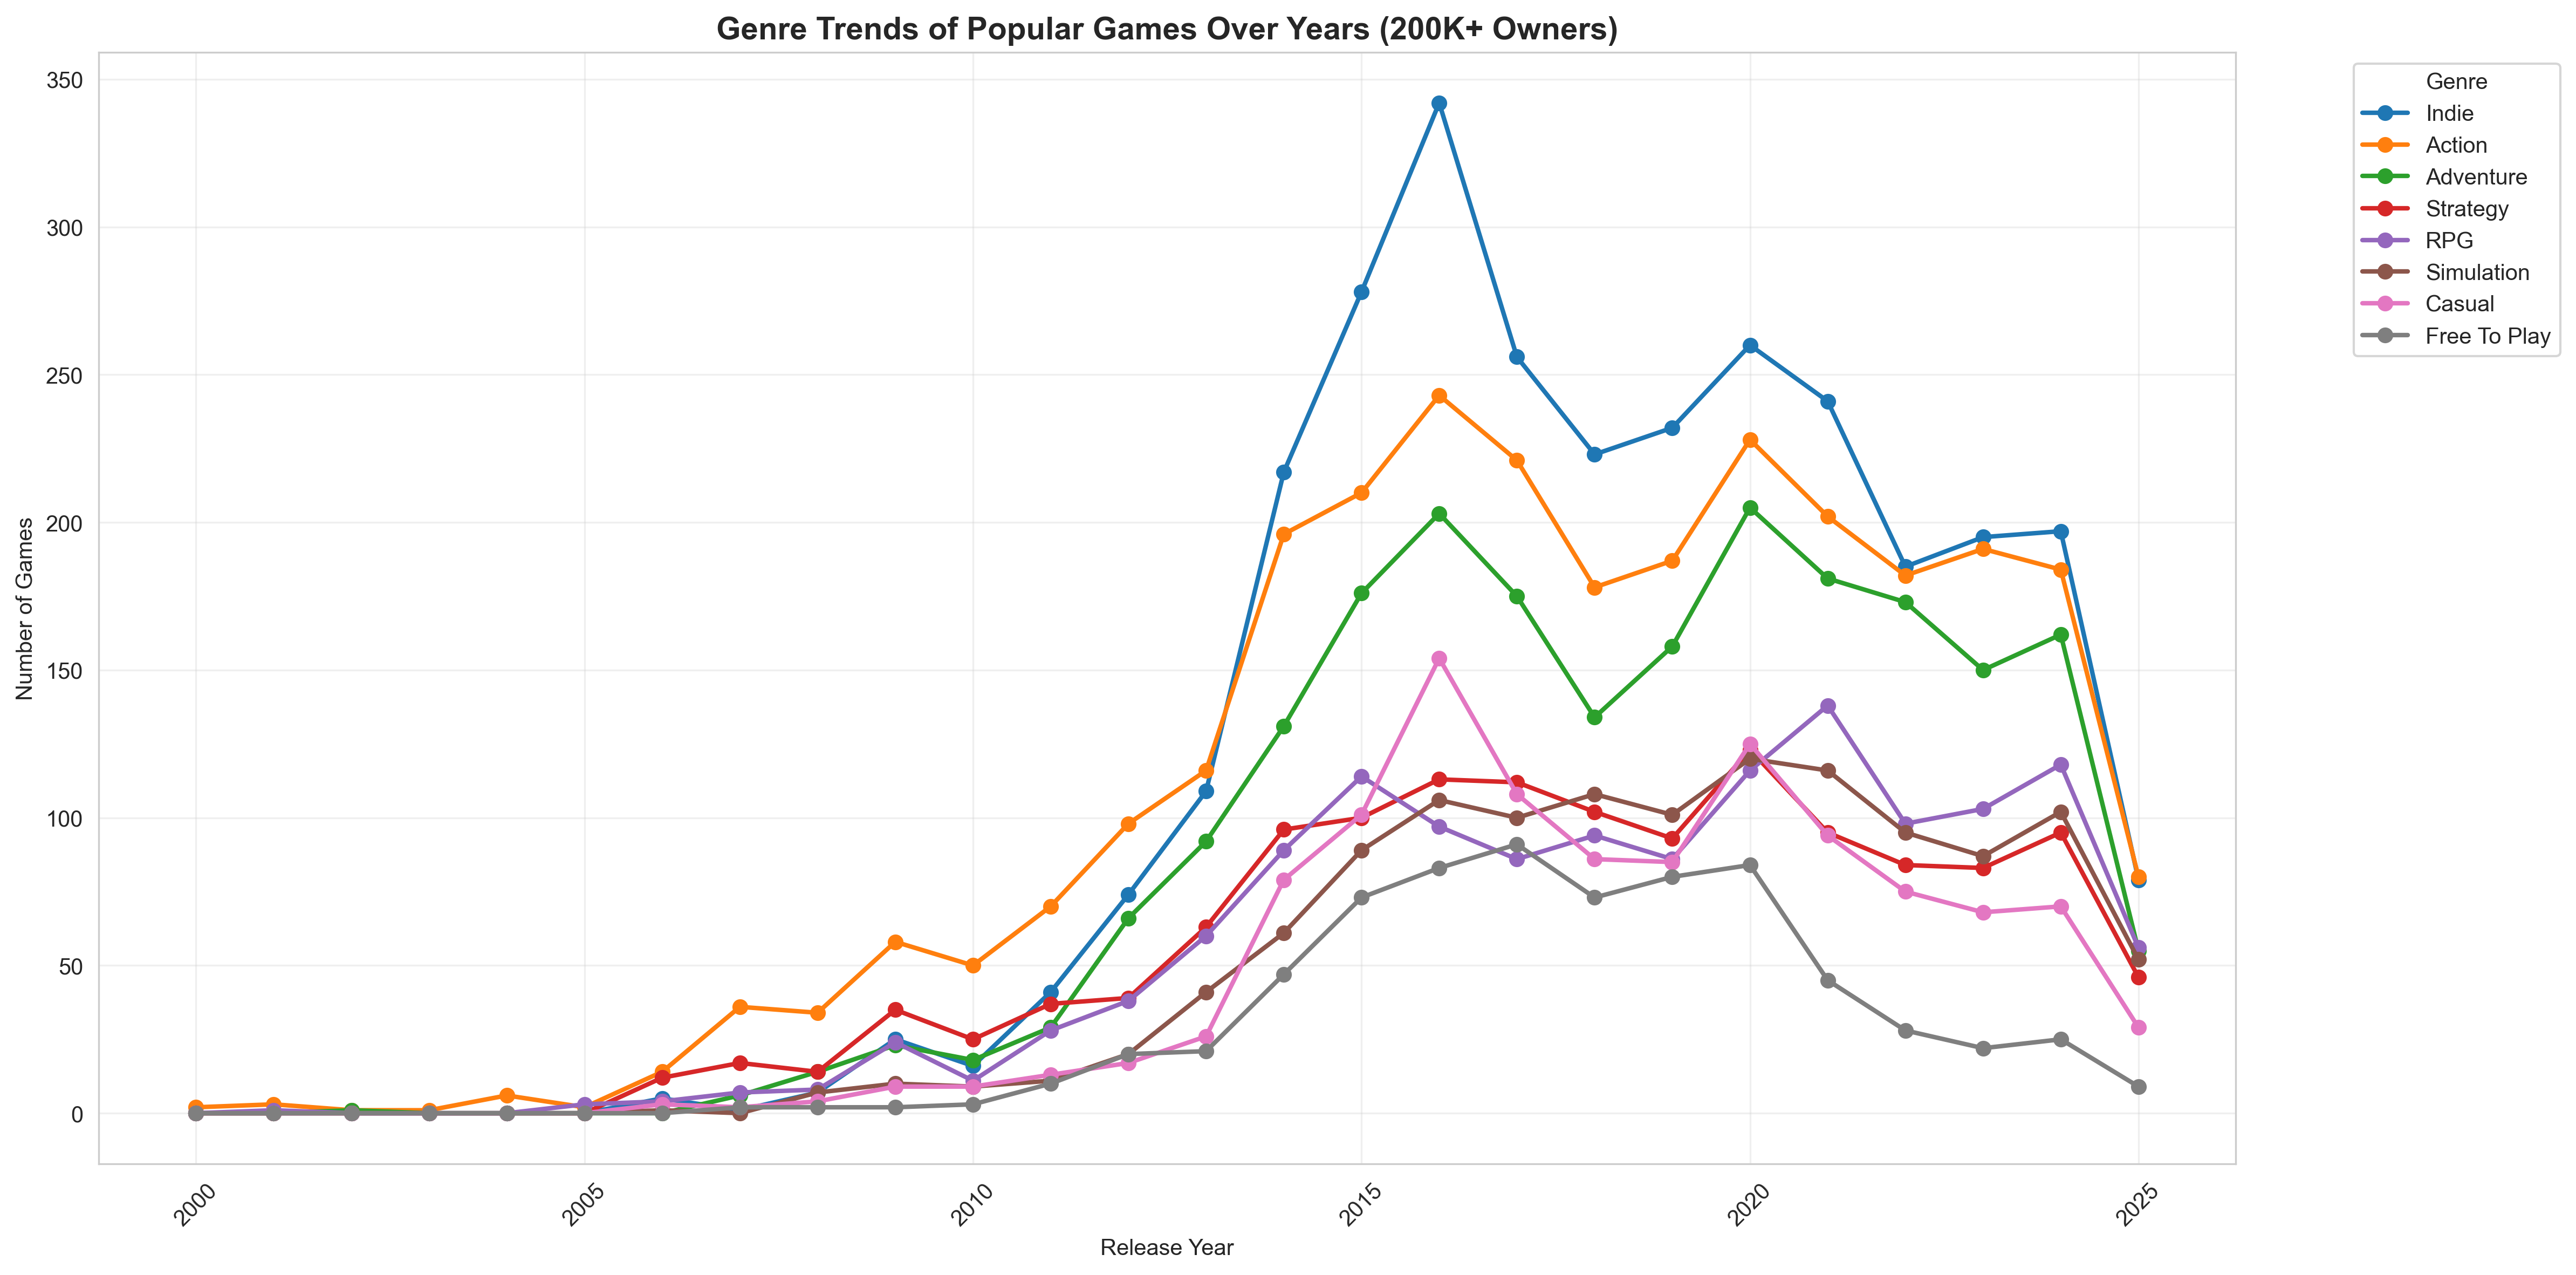
\includegraphics[width=0.48\linewidth]{Images/08_genre_trends_over_years.png}
    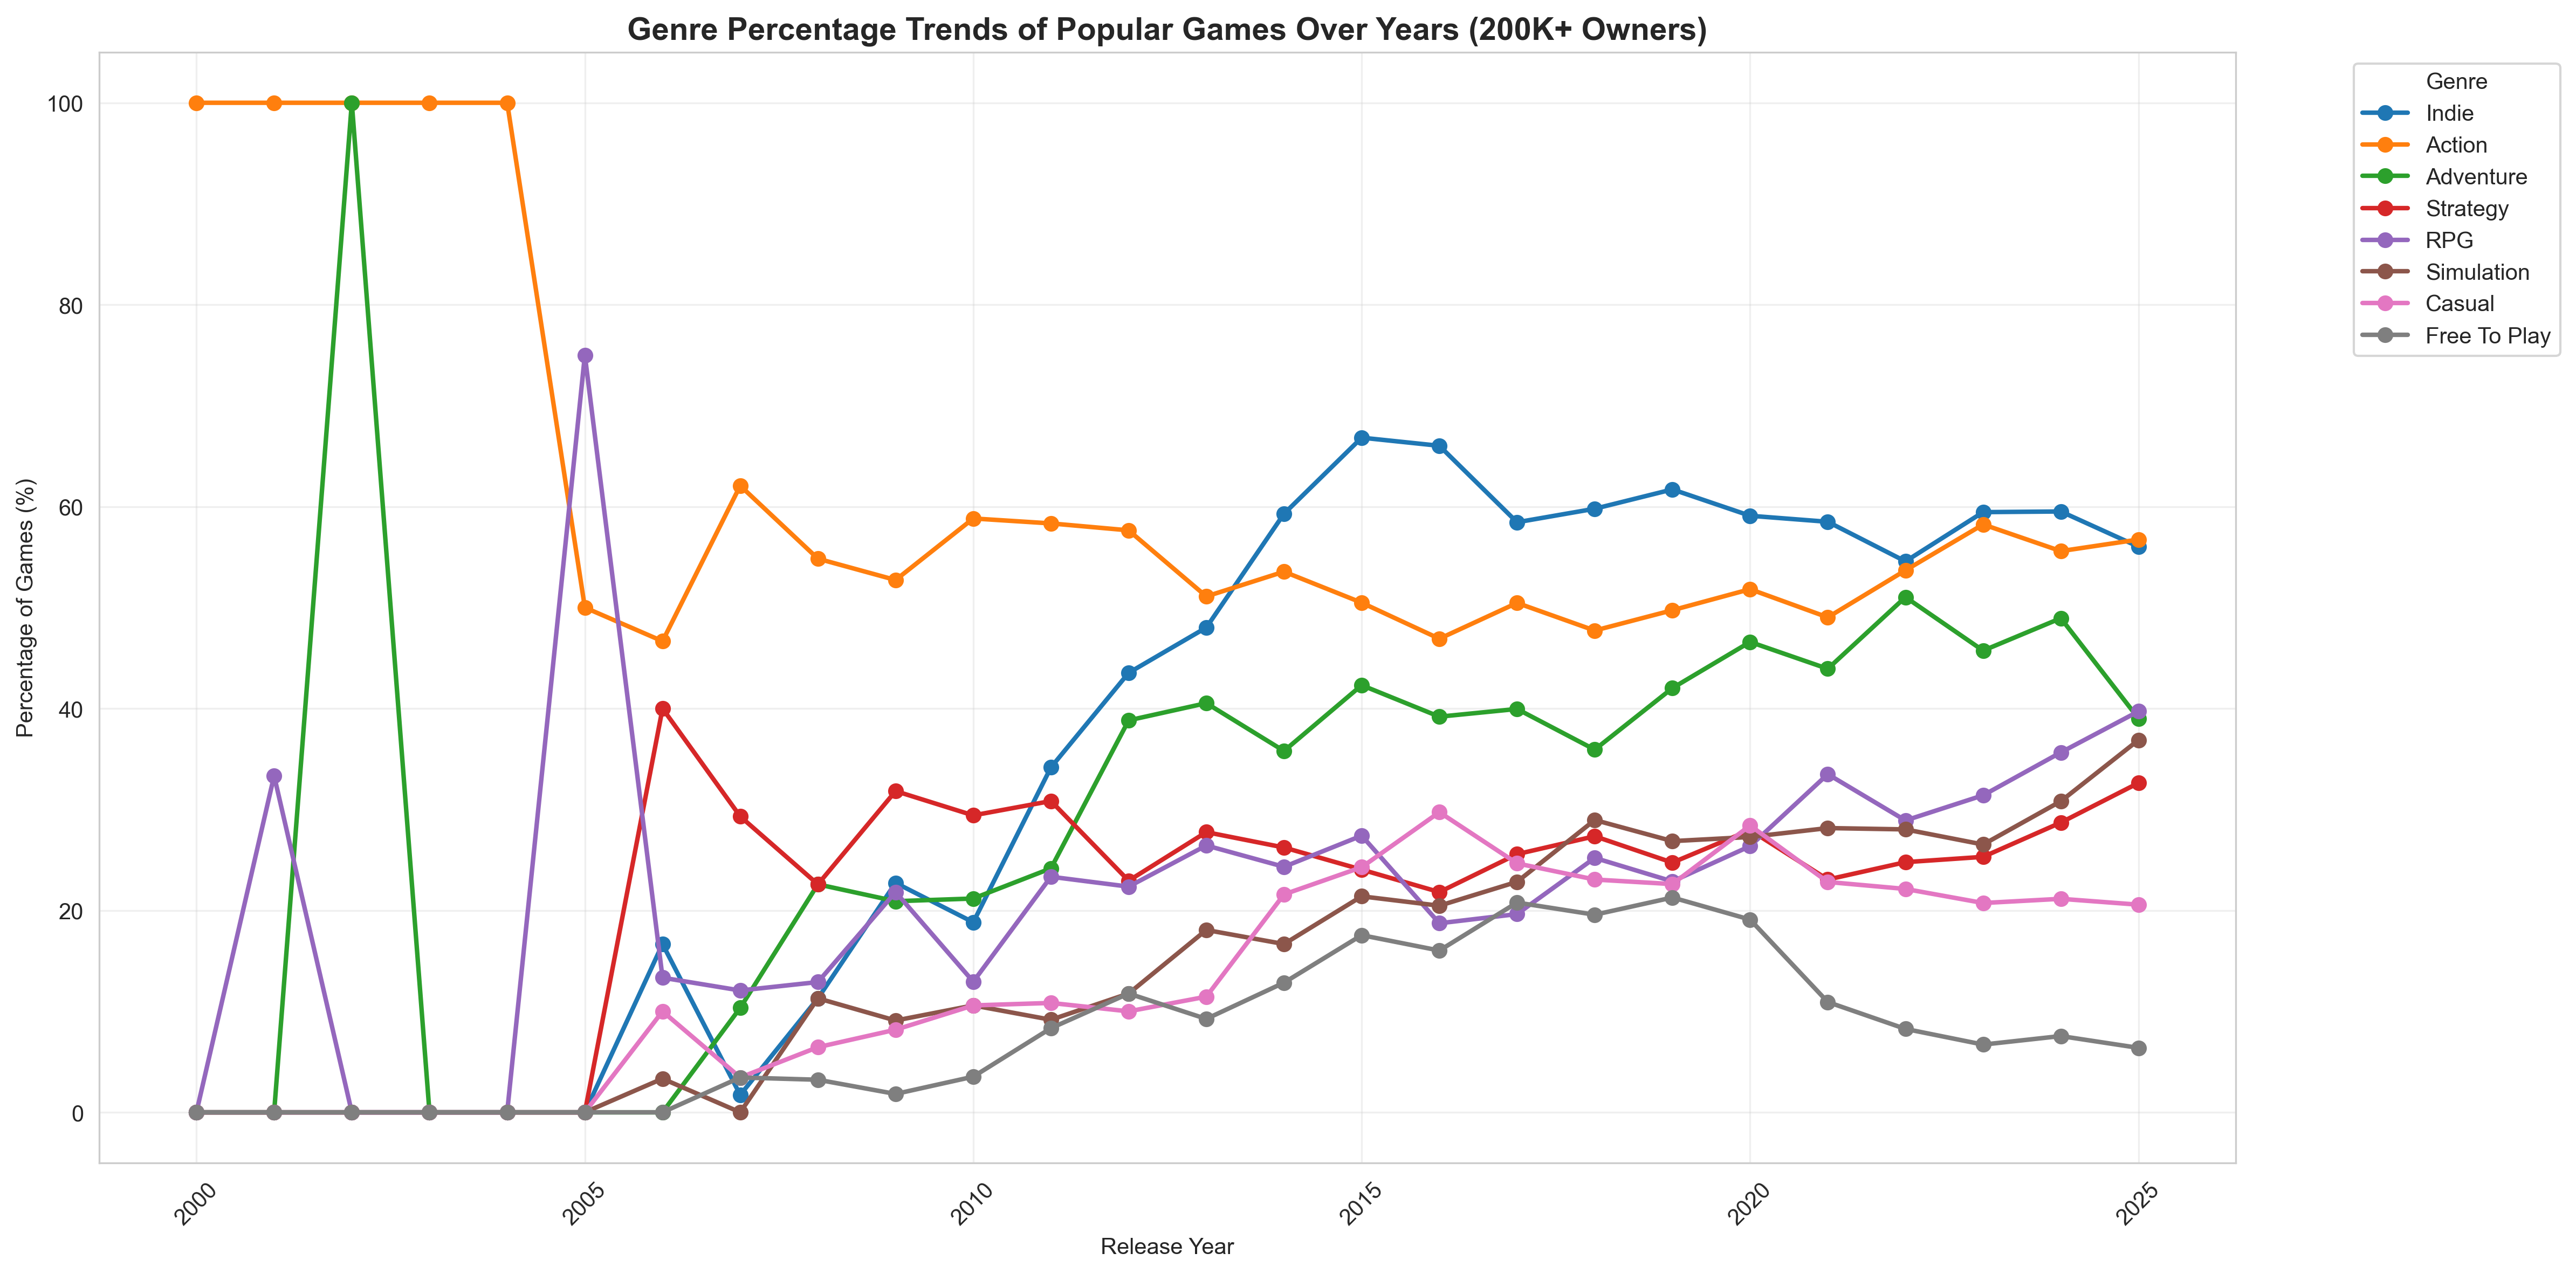
\includegraphics[width=0.48\linewidth]{Images/09_genre_percentage_trends.png}
    \caption{Xu hướng số lượng (trái) và tỷ lệ (phải) các thể loại game phổ biến (200K+) qua từng năm.}
    \label{fig:genre_trends_lines}
\end{figure}
\begin{figure}[H]
    \centering
    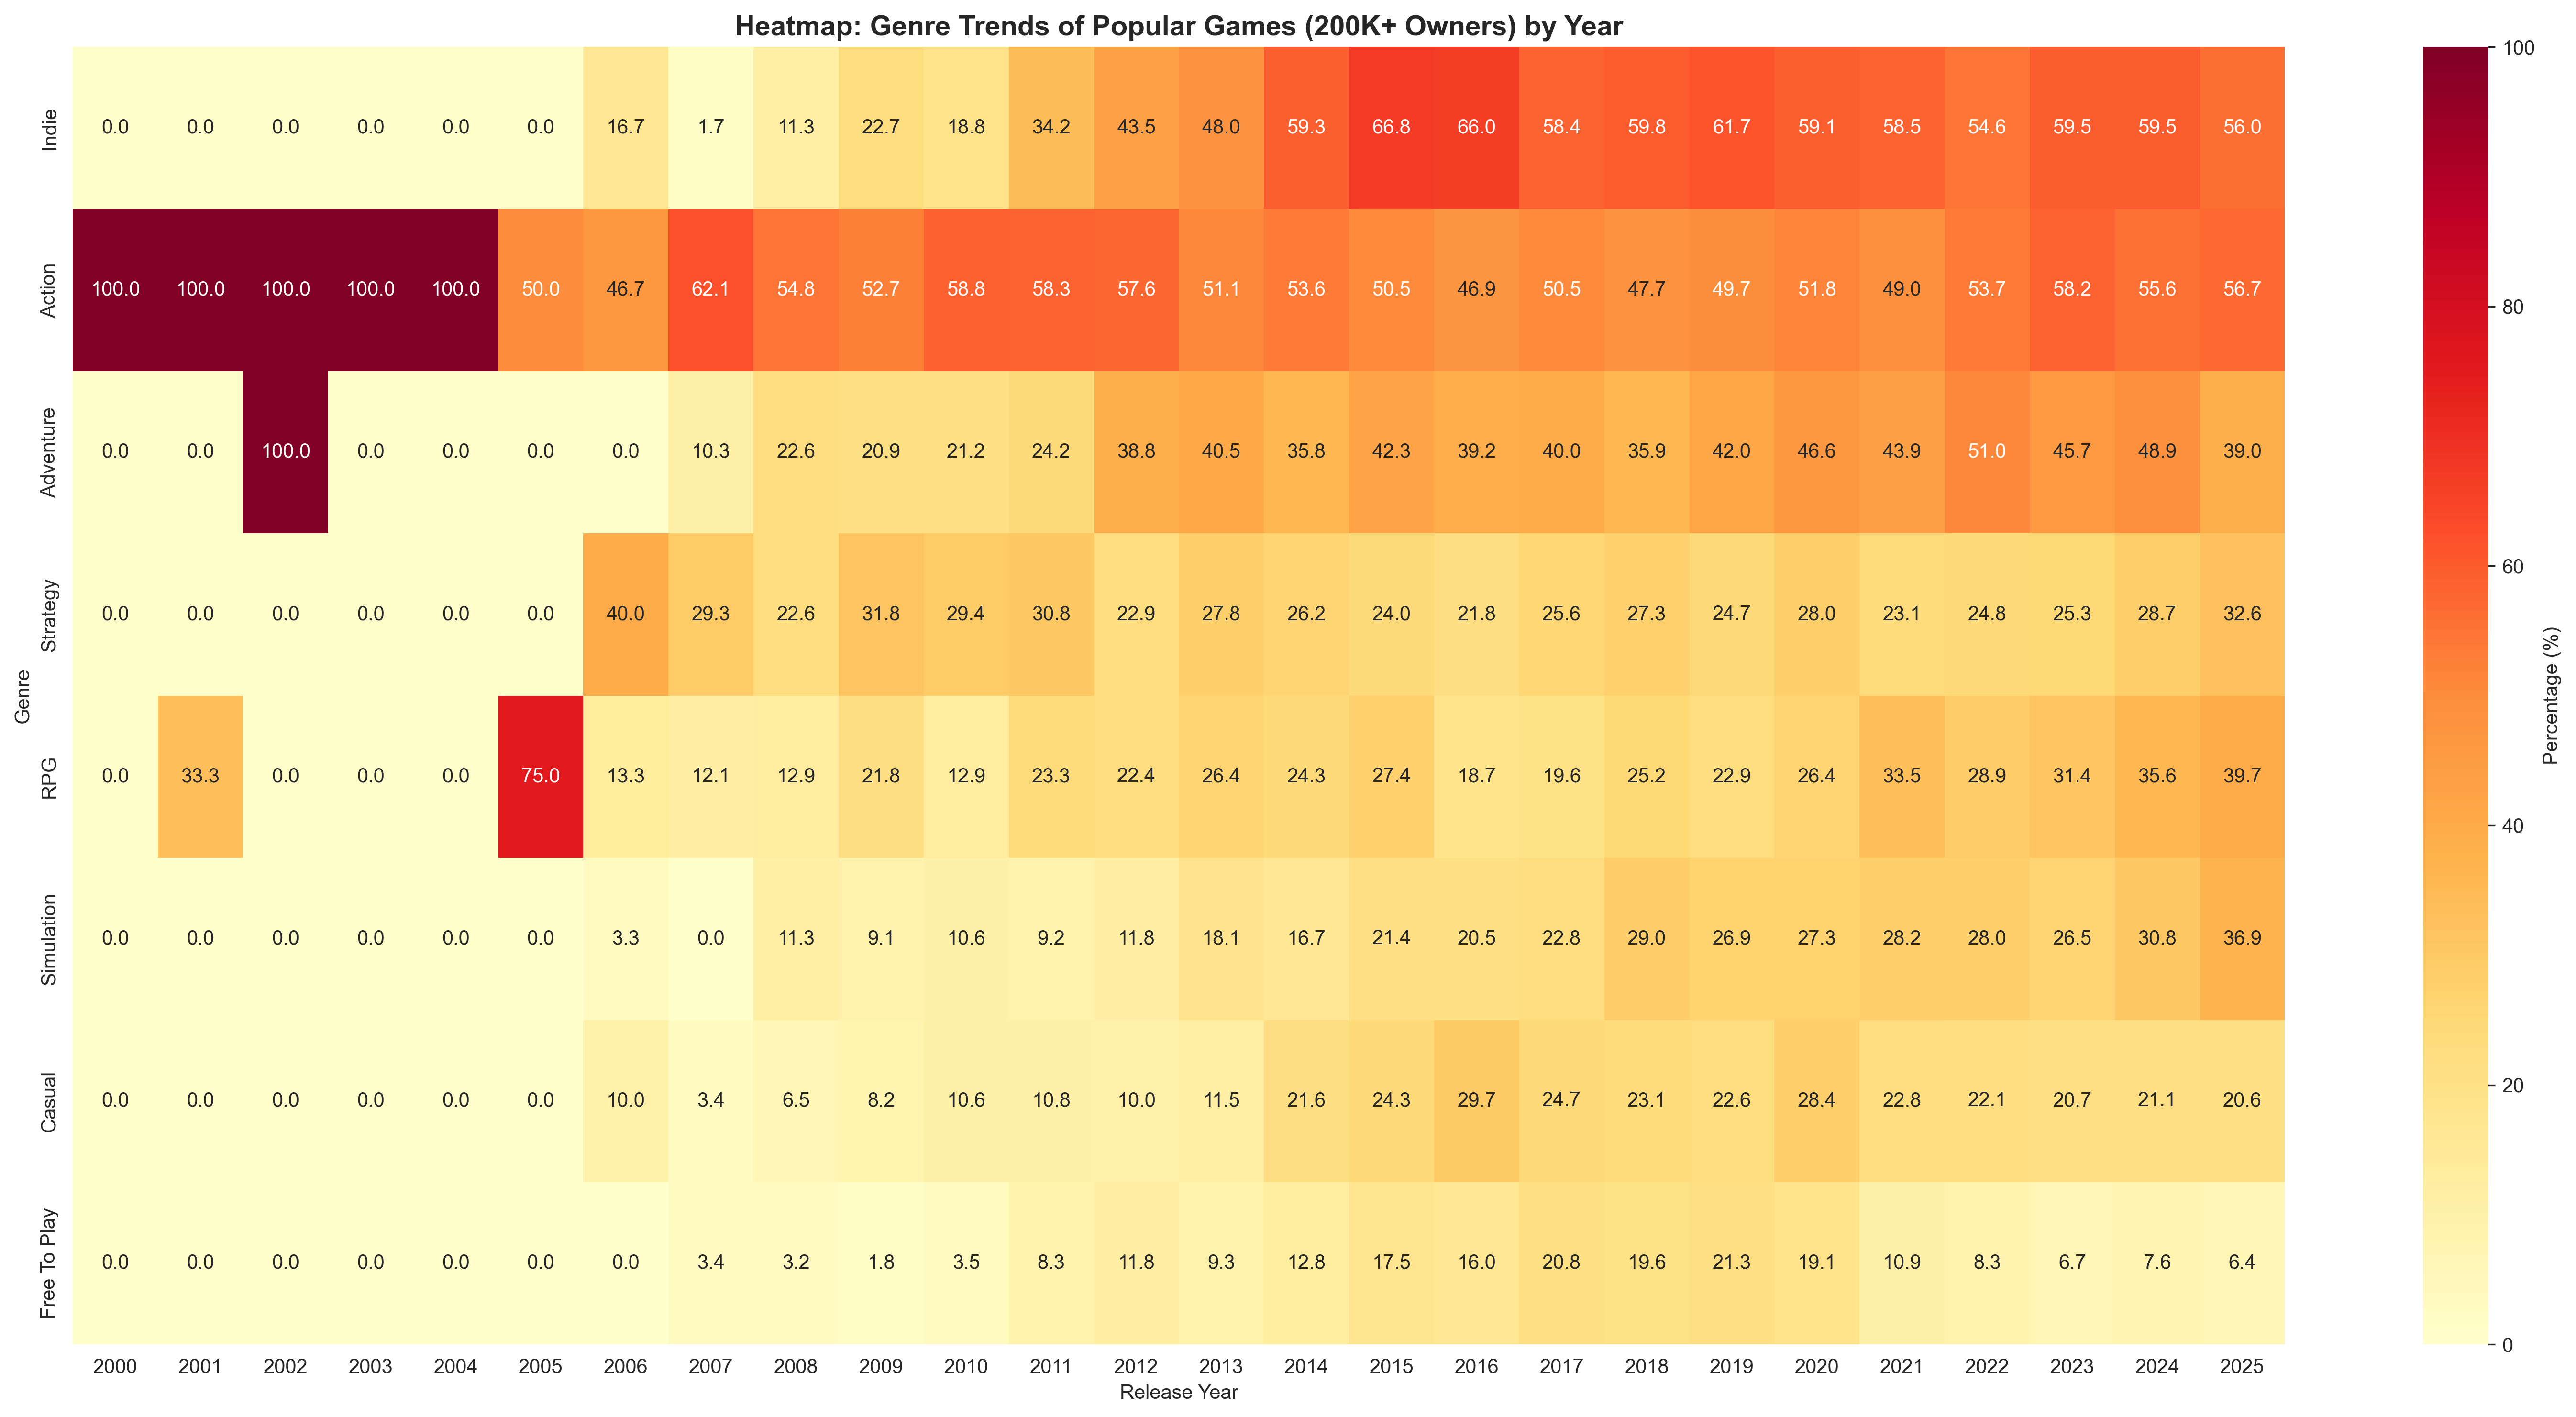
\includegraphics[width=0.8\linewidth]{Images/10_genre_trends_heatmap.png}
    \caption{Bản đồ nhiệt tỷ lệ thể loại game phổ biến (200K+) ra mắt theo năm.}
    \label{fig:10_genre_trends_heatmap}
\end{figure}
\hspace{1cm} Phân tích chuỗi thời gian đối với nhóm game thành công (trên 200.000 người sở hữu) ở Hình \ref{fig:genre_trends_lines} và Hình \ref{fig:10_genre_trends_heatmap} cung cấp cái nhìn lịch sử giá trị. Thể loại "Action" luôn là mỏ vàng ổn định nhất của ngành công nghiệp trong 25 năm qua. Tuy nhiên, hiện tượng bùng nổ ấn tượng nhất thuộc về dòng game "Indie".
\\

\hspace{1cm} Từ vị thế gần như không đáng kể trước năm 2005, Indie bắt đầu tăng tốc dần và bùng nổ dữ dội vào giai đoạn 2014-2018 (chiếm tới 60\% tổng số lượng game thành công mới ra mắt). Biểu đồ tỷ lệ (Hình \ref{fig:genre_trends_lines} phải) cũng cho thấy xu hướng đa dạng hóa (casual, RPG) đang dần lấy lại vị thế trong những năm gần đây (2020-2025). Những chuyển dịch này là minh chứng rõ nét cho kỷ nguyên "dân chủ hóa" công nghệ lập trình game, nơi các Engine miễn phí (như Unity, Godot) cho phép các nhóm nhỏ tạo ra những tựa game có thể cạnh tranh sòng phẳng trên thị trường quốc tế.






\newpage
\section{Kết luận và hướng phát triển}

\subsection{Kết luận}
\hspace{1cm} Trong bối cảnh ngành công nghiệp trò chơi điện tử đang phát triển với tốc độ vũ bão và tính cạnh tranh ngày càng khốc liệt, việc ra quyết định dựa trên cảm tính đã không còn mang lại hiệu quả. Bài báo cáo này đã thực hiện thành công một quy trình Khai phá dữ liệu (Data Mining) toàn diện trên một tập dữ liệu đồ sộ bao gồm hơn 122.000 trò chơi điện tử được phát hành trên nền tảng Steam trong suốt gần ba thập kỷ (từ năm 1997 đến năm 2025). Thông qua việc làm sạch, chuyển đổi và phân tích dữ liệu, nghiên cứu đã bóc tách được những quy luật ngầm ẩn, từ đó đánh giá chính xác quá trình phát triển của ngành công nghiệp game và đưa ra các định hướng chiến lược có giá trị thực tiễn cao.

\hspace{1cm} Về mặt phương pháp luận, nghiên cứu đã chứng minh được sức mạnh của việc kết hợp đa dạng các thuật toán học máy. Đối với bài toán Phân loại (Classification), các thuật toán như Decision Tree, Random Forest và SVM đã cho thấy khả năng vượt trội trong việc dự đoán tiềm năng thành công của một tựa game (đạt ngưỡng 200.000+ người sở hữu) dựa trên các đặc trưng như giá bán, thể loại, hệ điều hành hỗ trợ, độ dài mô tả và số lượng bản mở rộng (DLC). Đối với bài toán Gom cụm (Clustering), các thuật toán K-Means và DBSCAN đã làm tốt nhiệm vụ phân chia thị trường thành các phân khúc (market segments) rõ rệt, giúp định hình những ngách thị trường tiềm năng mà các studio độc lập (indie studios) có thể nhắm tới với chi phí thấp nhưng tỷ lệ thành công cao. Cuối cùng, việc ứng dụng Khai phá luật kết hợp (Association Rules Mining) thông qua Apriori và FP-Growth đã phát hiện ra các mẫu (patterns) hành vi thú vị, chẳng hạn như sự kết hợp hoàn hảo giữa các thể loại (như Action luôn đi kèm Adventure) hay quy luật định giá linh hoạt khi hỗ trợ đa nền tảng (game hỗ trợ Mac và có nhiều DLC thường có giá bán cao hơn).

\hspace{1cm} Từ kết quả của các mô hình và quá trình trực quan hóa dữ liệu, nghiên cứu rút ra những nhận định mang tính định hướng cho các nhà phát triển. Thứ nhất, mô hình kinh doanh "Free-to-Play" kết hợp với vi giao dịch đang là công cụ thâu tóm lượng người chơi mạnh mẽ nhất. Thứ hai, sự bùng nổ của dòng game Indie trong những năm gần đây minh chứng cho việc ý tưởng sáng tạo và lối chơi (gameplay) đột phá hoàn toàn có thể chiến thắng ngân sách đồ họa khổng lồ. Thứ ba, sự sống còn của một tựa game phụ thuộc tuyệt đối vào tỷ lệ đánh giá tích cực (Positive Reviews) từ cộng đồng, đòi hỏi các studio phải liên tục tương tác, cập nhật vá lỗi và lắng nghe người dùng. 

\hspace{1cm} Tóm lại, kết quả của đề tài không chỉ dừng lại ở góc độ học thuật mà còn đóng vai trò như một bản thiết kế chiến lược. Nó giúp các nhà quản lý, các nhà thiết kế game (Game Designers) và đặc biệt là các Indie Studios tối ưu hóa sản phẩm từ khâu lên ý tưởng thể loại, lập kế hoạch phát triển đa nền tảng, cho đến chiến lược định giá nhằm giảm thiểu rủi ro tài chính và tối đa hóa khả năng tiếp cận người chơi.

\subsection{Hướng phát triển}
\hspace{1cm} Mặc dù đã đạt được những kết quả phân tích khả quan và giải quyết được các mục tiêu ban đầu của đề tài, bài toán khai phá dữ liệu ngành game vẫn còn rất nhiều không gian để mở rộng và đào sâu. Để nâng cao độ chính xác của các mô hình dự đoán và cung cấp những công cụ đắc lực hơn nữa cho các nhà phát triển, nhóm đề xuất các hướng phát triển trong tương lai như sau:

\begin{itemize}
    \item \textbf{Khai phá dữ liệu văn bản chuyên sâu (Advanced Text Mining \& NLP):} Thay vì chỉ sử dụng số lượng đánh giá tích cực và tiêu cực như các biến số vô tri, hệ thống có thể được nâng cấp để đọc hiểu ngôn ngữ tự nhiên. Bằng cách áp dụng các mô hình học sâu (Deep Learning) như BERT hay Transformer vào cột \texttt{Reviews} và \texttt{About the game}, ta có thể thực hiện Phân tích cảm xúc (Sentiment Analysis) và Mô hình hóa chủ đề (Topic Modeling). Điều này sẽ giúp studio biết chính xác người chơi đang phàn nàn về điều gì (ví dụ: cốt truyện nhàm chán, đồ họa lỗi, hay cơ chế điều khiển khó) để có phương án sửa chữa kịp thời.
    
    \item \textbf{Dự báo chuỗi thời gian và vòng đời sản phẩm (Time-series Forecasting):} Áp dụng các thuật toán dự báo mạnh mẽ như ARIMA, Prophet hoặc Mạng bộ nhớ dài-ngắn (LSTM) để phân tích dữ liệu lượng người chơi đồng thời (Peak CCU) thay đổi theo từng ngày. Hướng đi này giúp dự đoán được "tuổi thọ" của một tựa game, thời điểm lượng người chơi bắt đầu suy giảm (churn rate) để nhà phát hành tung ra các bản cập nhật (Update), gói mở rộng (DLC) hoặc các chương trình giảm giá (Discount) nhằm kéo cộng đồng quay trở lại.
    
    \item \textbf{Xây dựng Hệ tư vấn (Recommendation Systems):} Tận dụng kết quả từ thuật toán Gom cụm (Clustering) và Khai phá luật kết hợp (Association Rules) để xây dựng một hệ thống tư vấn thông minh (Collaborative Filtering hoặc Content-based). Hệ thống này không chỉ dùng để gợi ý game cho người chơi (như cách Steam đang làm), mà còn có thể tư vấn ngược lại cho các nhà phát triển. Ví dụ: khi một lập trình viên nhập vào hệ thống ý tưởng "Game nhập vai (RPG), đồ họa Pixel, giá 5\$", hệ thống sẽ gợi ý "Bạn nên hỗ trợ thêm hệ điều hành Linux và thêm thẻ (Tag) Co-op để tăng 15\% cơ hội thành công".
    
    \item \textbf{Mở rộng và tích hợp đa nguồn dữ liệu (Cross-platform Data Integration):} Thị trường game không chỉ gói gọn trong Steam. Trong tương lai, tập dữ liệu có thể được làm phong phú hơn bằng cách cào dữ liệu (Web Scraping) hoặc kết nối API với các nền tảng phân phối khác như Epic Games Store, PlayStation Network, Xbox Live. Ngoài ra, việc kết hợp với dữ liệu lượt xem từ nền tảng phát trực tiếp (như Twitch, YouTube Gaming) sẽ tạo ra một biến số mới cực kỳ quan trọng để đánh giá mức độ lan truyền (viral) của tựa game.
    
    \item \textbf{Triển khai thành ứng dụng thực tế (Model Deployment \& MLOps):} Đóng gói các mô hình Machine Learning đã được huấn luyện thành một dịch vụ Web (Web Service) hoàn chỉnh thông qua các framework như FastAPI, Flask hoặc Streamlit. Giao diện trực quan này sẽ cho phép các studio game, nhà đầu tư nhập các thông số dự kiến của dự án game sắp phát hành và nhận về một bản báo cáo phân tích rủi ro, dự đoán doanh thu cũng như xác suất thành công theo thời gian thực.
\end{itemize}






\newpage

\begin{thebibliography}{9}
    \bibitem{dataset_steam} Fronkon Games, ``Steam Games Dataset,'' \textit{Kaggle}. [Online]. Đường dẫn: \url{https://www.kaggle.com/datasets/fronkongames/steam-games-dataset}.
\end{thebibliography}
